\documentclass[10pt]{beamer}

\usetheme{metropolis}
\usepackage{appendixnumberbeamer}

\usepackage{graphicx}
\graphicspath{ {../img/} }

\usepackage{booktabs} % Allows the use of \toprule, \midrule and \bottomrule in tables
\newcommand{\tabitem}{~~\llap{\textbullet}~~}
\usepackage[scale=2]{ccicons}

\usepackage{pgfplots}
\usepgfplotslibrary{dateplot}

\usepackage{xspace}
\newcommand{\themename}{\textbf{\textsc{metropolis}}\xspace}

\usepackage{tikz}
\usetikzlibrary{shapes.geometric, arrows, fit, positioning, calc}
\tikzstyle{data} = [rectangle, rounded corners, minimum width=2.5cm, minimum height=0.8cm, text centered, text width=2.5cm, draw=black, fill=blue!30]

\usepackage{relsize}
\tikzset{fontscale/.style = {font=\relsize{#1}}}

\usepackage{multirow}

\usepackage{color}
\newcommand{\tc}[1]{\textcolor{red}{#1}}

{%
\fboxsep=0pt
\fboxrule=2pt
}%

%----------------------------------------------------------------------------------------
% TITLE PAGE
%----------------------------------------------------------------------------------------
\title[Interface of 3D Reconstruction]{Development and Application of a Description-based Interface for 3D Reconstruction} % The short title appears at the bottom of every slide, the full title is only on the title page

\author{Kai Wu}
\institute[UBC]
{
University of British Columbia \\ % Your institution for the title page
\medskip
kaywu@ece.ubc.ca \\ % Your email address
}
\date{\today}

\begin{document}

\begin{frame}
\maketitle
\end{frame}

\begin{frame}{Table of contents}
  \setbeamertemplate{section in toc}[sections numbered]
  \tableofcontents[hideallsubsections]
\end{frame}

%----------------------------------------------------------------------------------------
% PRESENTATION SLIDES
%----------------------------------------------------------------------------------------

%------------------------------------------------
\section{Introduction}
%------------------------------------------------
\begin{frame}{Motivation: application}

\begin{figure}
\centering
\begin{tabular}{*{3}{p{3.2cm}}}
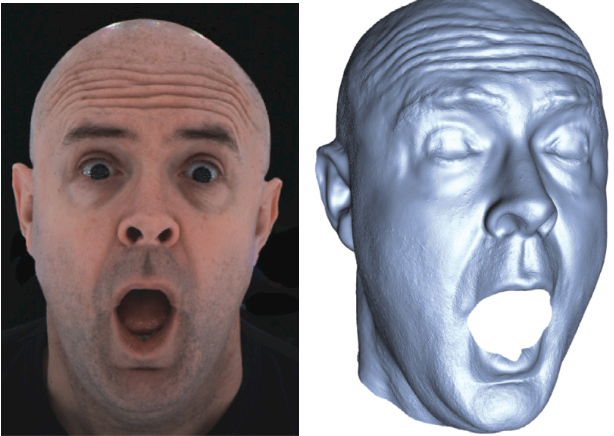
\includegraphics[width=0.3\textwidth]{images/visual_effects.png} &
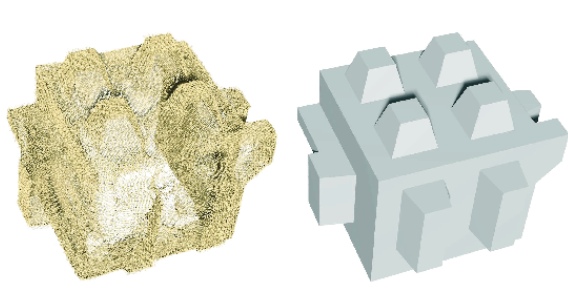
\includegraphics[width=0.3\textwidth]{images/inverse_cad.png} &
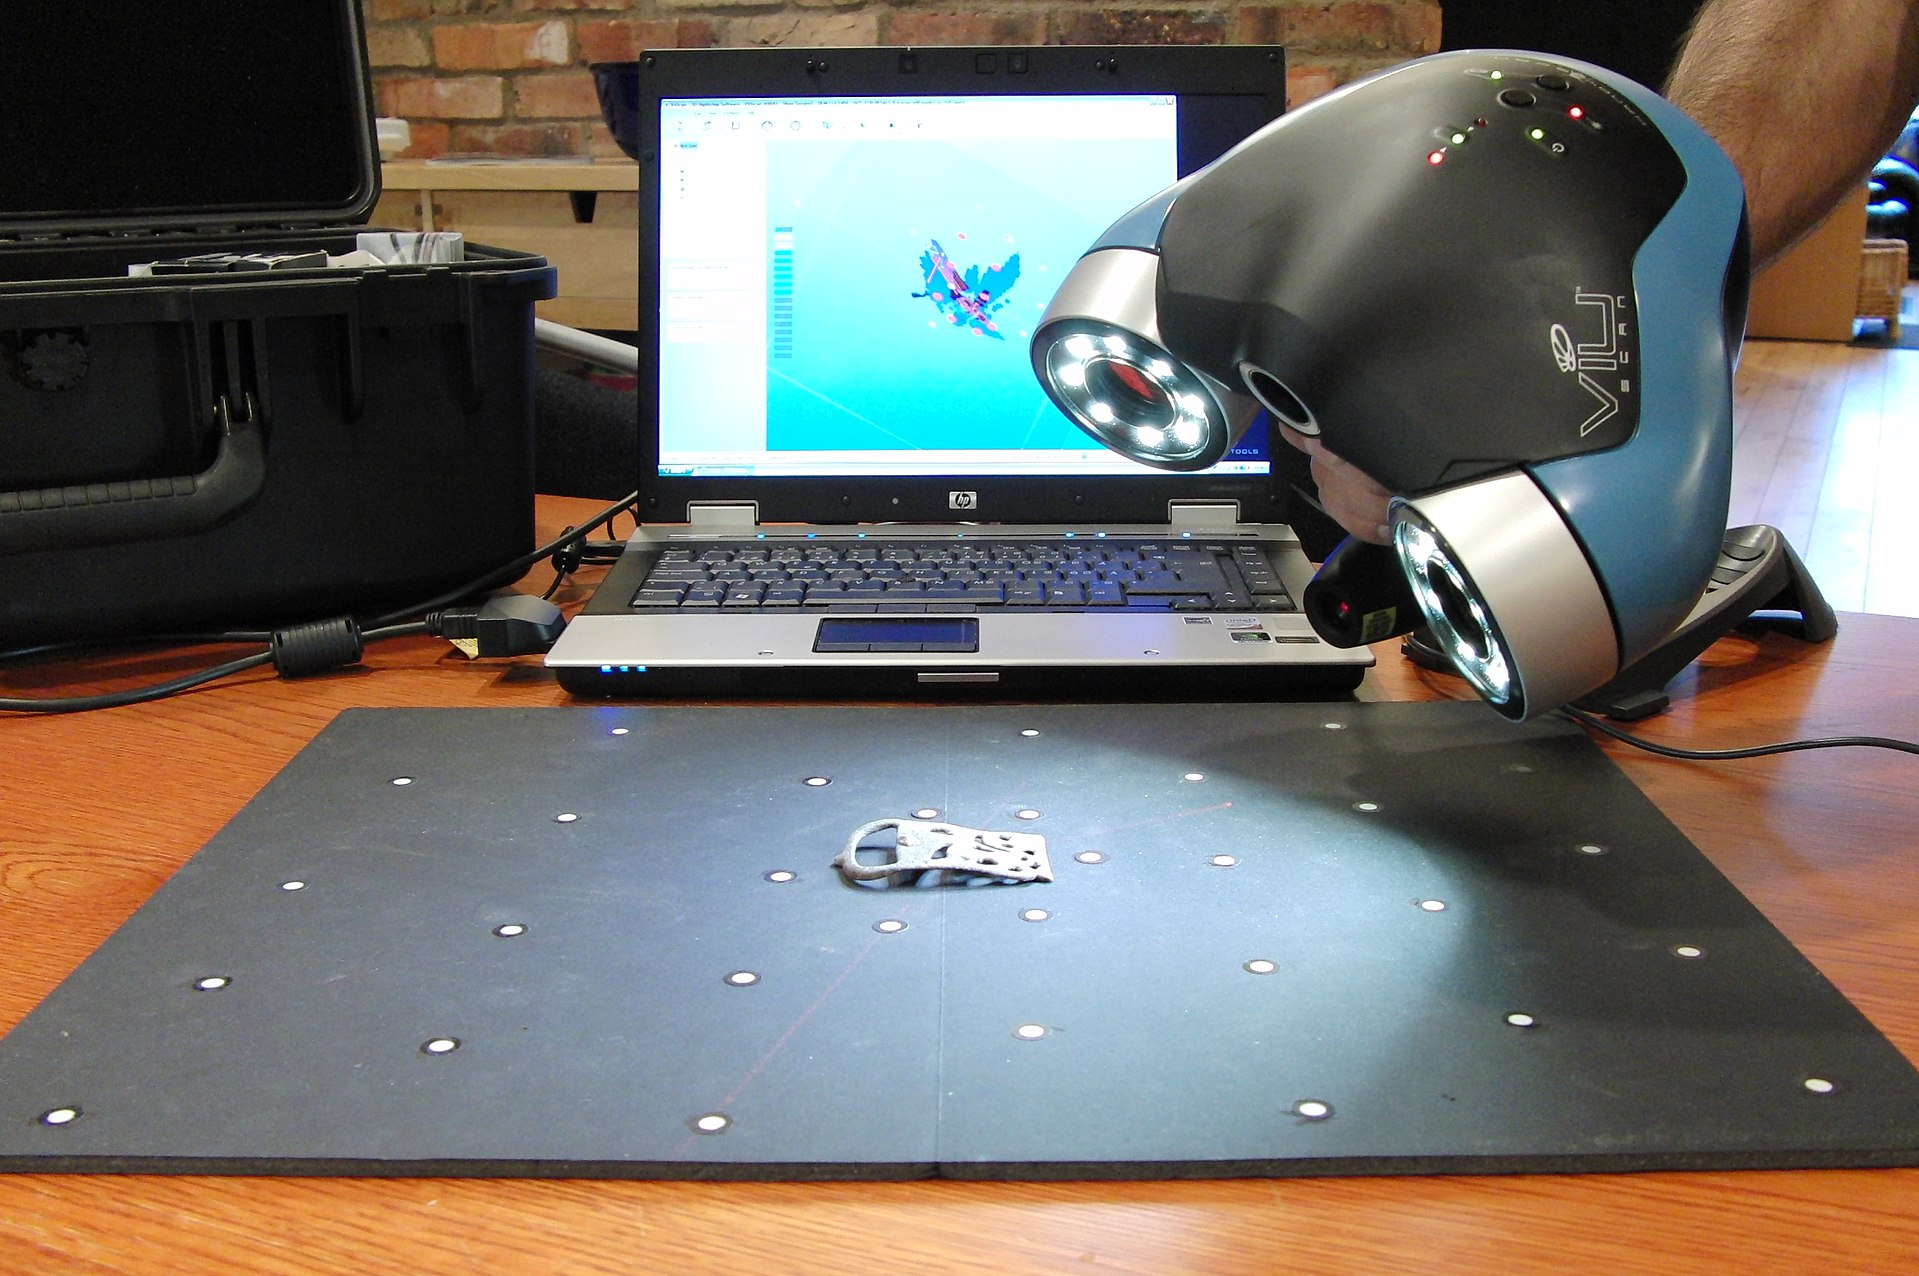
\includegraphics[width=0.3\textwidth]{images/3d_scanner.jpg} \\
Visual effects & Inverse CAD & 3D scanner \\
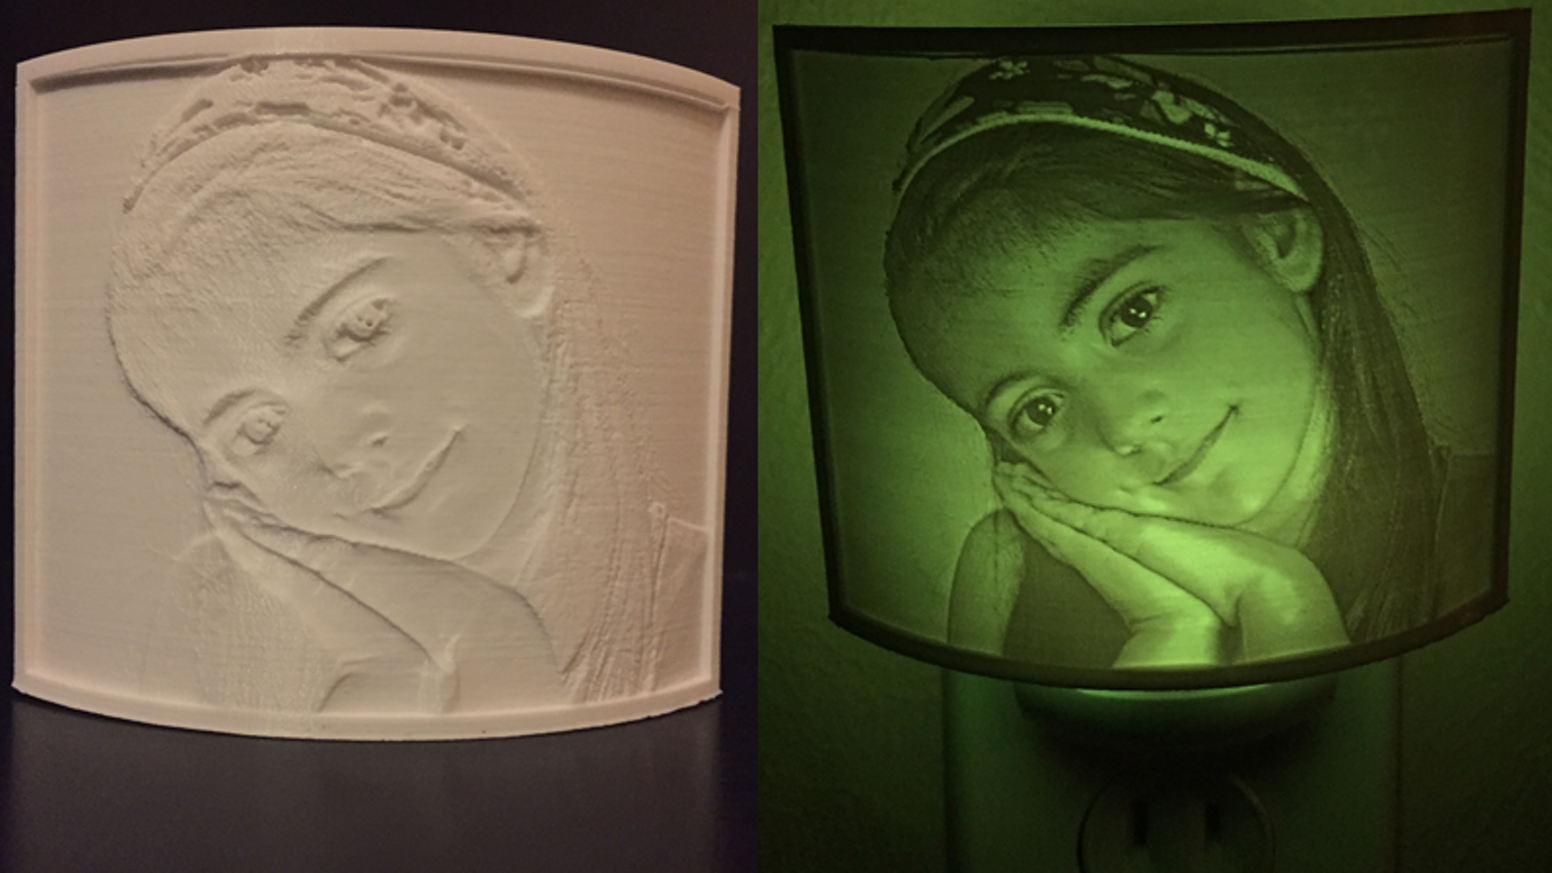
\includegraphics[width=0.3\textwidth]{images/customization.png} & 
\\
Customization & DIY Repair\& Reconstruction & Virtual content creation \\
\end{tabular}
\end{figure}
% \begin{itemize}
% \item digital mapping
% \item visual effects
% \item virtual content creation
% \item 3D artist
% \item inverse CAD
% \item 3D printing's counterpart: 3D scanner
% \end{itemize}
\end{frame}

%------------------------------------------------
\begin{frame}{Motivation: traditional 3D reconstruction}

\begin{figure}
\centering
\includegraphics[width=0.9\textwidth]{images/3d_recon_traditional_2.pdf}
\end{figure}

\begin{alertblock}{Challenges}
  \begin{itemize}
    \item \textbf{Algorithms}: vision knowledge required;
    \item \textbf{Parameters}: not interpretable, meaningful, or conceptually estimatible;
    \item \textbf{Approach}: \textit{trial-and-error}.
  \end{itemize}
\end{alertblock}

\end{frame}

%------------------------------------------------
\begin{frame}{Goal}

\begin{table}
\centering
\begin{tabular}{l|*{2}{p{4cm}}}
& Traditional 3D Recon & Interface for 3D Recon\\
\midrule
Algorithm & vision knowledge & hidden \\
Parameter & algorithm-specific params & params of visual\& geometric properties \\
Approach & multiple trial-and-error & no trial-and-error \\
\end{tabular}
\end{table}

\end{frame}

%------------------------------------------------
\begin{frame}{Contribution}

Development of an interface for 3D reconstruction problem, which hides algorithm details and allows users to describe conditions surrounding the problem. This description can be interpreteded so that an appropriate algorithm is chosen to achieve a successful reconstruction result.

\end{frame}

%------------------------------------------------
% \begin{frame}{Contribution (cont'd)}

% This contribution is significant because:
% \begin{itemize}
% \item Few algorithms can work for a diverse categories of objects. The interface, to some extent, can cover a wider range of object categories by incorporating multiple algorithms.
% \item An description of object problem condition is provided to hide the algorithmic details, thus understanding of the algorithm, or conditions of applying algorithms are not a prerequisite.
% \end{itemize}

% \end{frame}

%------------------------------------------------
\begin{frame}{Overview of thesis/presentation}

\begin{figure}
\centering
\includegraphics[width=\textwidth]{images/overview.pdf}
\end{figure}

\end{frame}

%------------------------------------------------
\section{Related Work}
%------------------------------------------------
\begin{frame}{Related Work: softwares}

% Some noteable open source general vision libraries and softwares:

\begin{exampleblock}{General vision libraries}
\begin{itemize}
  \item Example: OpenCV, VXL, VLFeat, and so on
  \item Problem: provide APIs for vision routines
\end{itemize}
\end{exampleblock}

\begin{exampleblock}{3D vision softwares}
  \begin{itemize}
    \item Example: PMVS; Bundler, VisualSfM, TheiaSfM; Poisson Recon;
    \item Problem: cater to specific objects, not applicable for textureless surface
  \end{itemize}
\end{exampleblock}

\begin{alertblock}{Challenges}
1. Not that we don't have enough tools, but the barrier to take advantage of these tools is high. \\
\end{alertblock}

\end{frame}

%------------------------------------------------
\begin{frame}{Related Work: algorithms}

\begin{exampleblock}{Shape from Stereo}
  \begin{itemize}
    \item Example: Multi-View Stereo, Structured Light
    \item Problem: Texture, reflectance
  \end{itemize}
\end{exampleblock}

\begin{exampleblock}{Shape from Intensity}
  \begin{itemize}
    \item Example: Shape from Shading, Photometric Stereo
    \item Problem: Lightness, shape
  \end{itemize}
\end{exampleblock}

\begin{exampleblock}{Shape from Silhouette}
  \begin{itemize}
    \item Example: Visual Hull, Space Carving
    \item Problem: Shape, reflectance
  \end{itemize}
\end{exampleblock}

% \begin{figure}
% \begin{tabular}{lll}
% \toprule
% Class & Method & Problem \\
% \midrule
% \multirow{2}{*}{Shape from Stereo} & 
% Multi-View Stereo &
% \multirow{2}{*}{Texture, reflectance} \\
% & Structured Light \\
% \multirow{2}{*}{Shape from Intensity} & 
% Shape from Shading & 
% \multirow{2}{*}{Lightness, shape} \\
% & Photometric Stereo \\
% \multirow{2}{*}{Shape from Silhouette} &
% Visual Hull & 
% \multirow{2}{*}{Shape, reflectance}\\
% & Space Carving \\
% \bottomrule
% \end{tabular}
% \end{figure}

% \begin{figure}
% \begin{tabular}{ccc}
% \toprule
% Class & Method & Problem \\
% \midrule
% \multirow{2}{*}{Shape from Stereo} & 
% \raisebox{-.5\height}{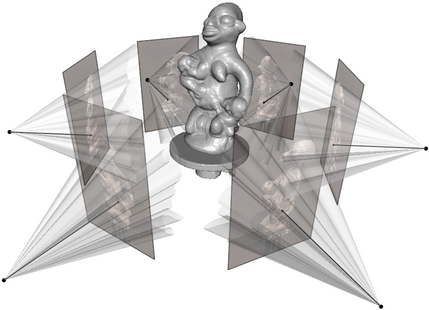
\includegraphics[height=1cm]{images/mvs.png}} &
% Texture, Specular \\
% &  \raisebox{-.5\height}{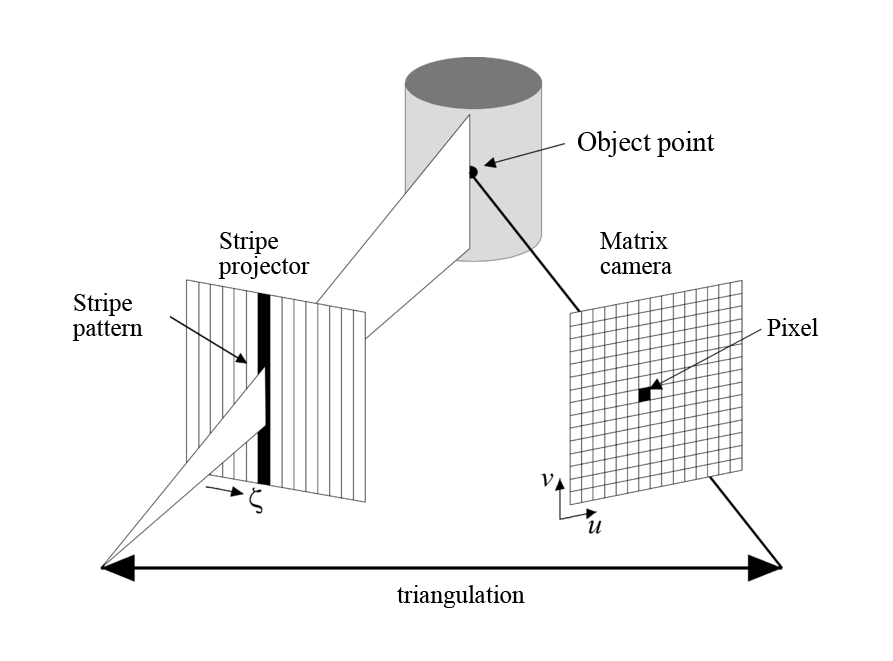
\includegraphics[height=1cm]{images/sl.jpg}} &
% Albedo, Specular \\
% \multirow{2}{*}{Shape from Intensity} & 
% \raisebox{-.5\height}{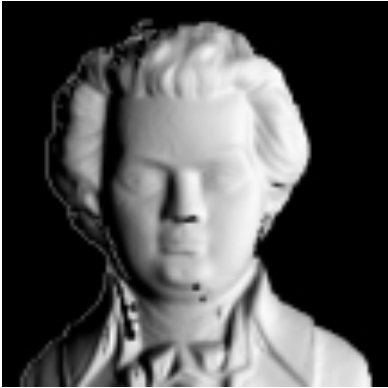
\includegraphics[height=1cm]{images/sfs.png}} &
% Albedo, Specular, Geomtry \\
% & \raisebox{-.5\height}{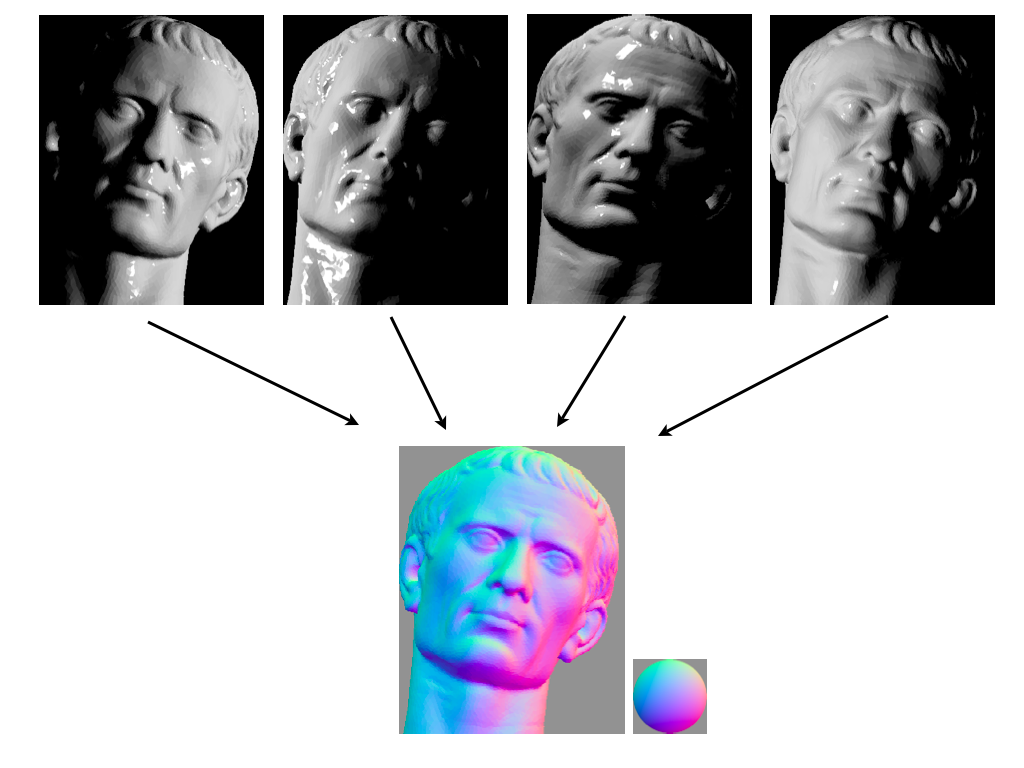
\includegraphics[height=1cm]{images/ps.png}} &
% Albedo, Geoemtry \\
% \multirow{2}{*}{Shape from Silhouette} &
% \raisebox{-.5\height}{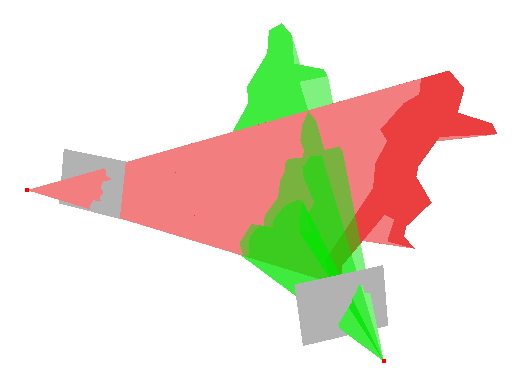
\includegraphics[height=1cm]{images/vh.jpg}} &
% Geoemtry\\
% & \raisebox{-.5\height}{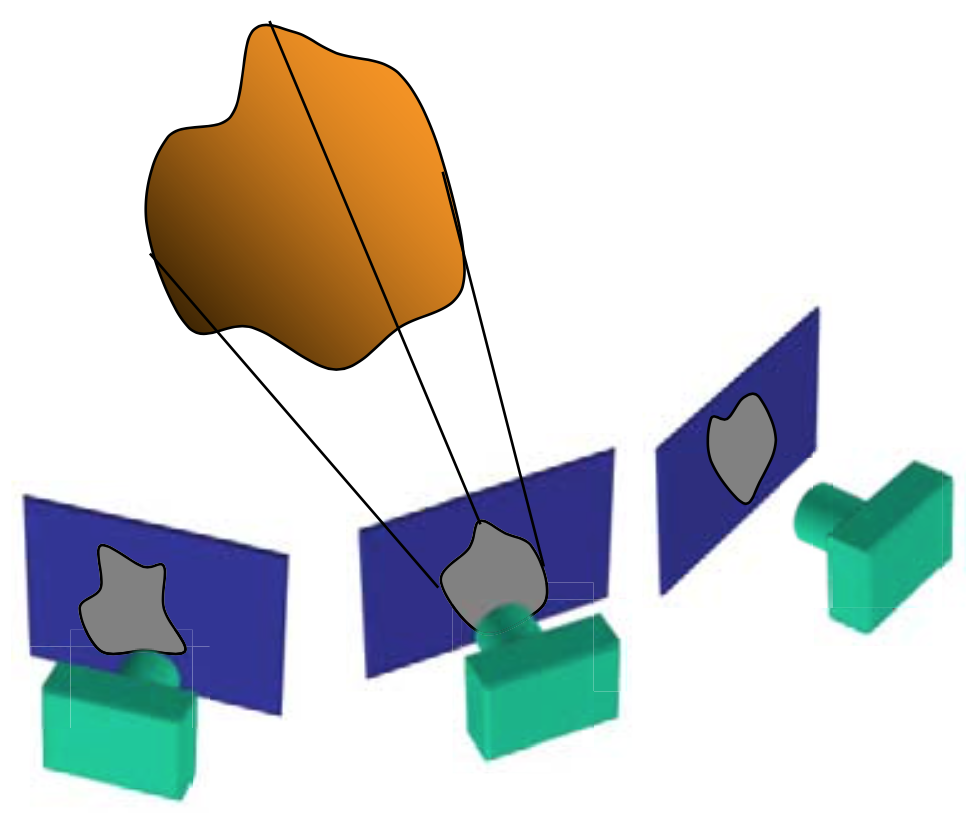
\includegraphics[height=1cm]{images/vh_1.png}} &
% Geoemtry\\
% \bottomrule
% \end{tabular}
% \end{figure}

\begin{alertblock}{Challenges}
1. Few algorithm works for objects with diverse range of properties;\\
2. The range of problem conditions under which an algorithm works is not known a priori.
\end{alertblock}

\end{frame}

%------------------------------------------------
\section{Development of Interface}
%------------------------------------------------
\begin{frame}{Overview of interface}
\begin{figure}
\centering
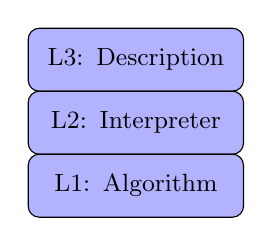
\begin{tikzpicture}[node distance=0.8cm, auto]

\node (desc) [data, font=\small] {L3: Description};
\node (interp) [data, below of=desc, font=\small] {L2: Interpreter};
\node (algo) [data, below of=interp, font=\small] {L1: Algorithm};

\end{tikzpicture}
\caption{3-layer interface to 3D reconstruction.}
\end{figure}

\begin{exampleblock}{Description}
  1. define problem space; \\
  2. describe problem condition.
\end{exampleblock}
\begin{exampleblock}{Interpreter: translate description to an appropriate algorithm.}
  Mapping: discover the relation between problem space and algorithm.
\end{exampleblock}
\begin{exampleblock}{Algorithm}
  Embed algorithms into the interface
\end{exampleblock}

\end{frame}

%------------------------------------------------
\subsection{Problem Space of 3D Reconstruction}
%------------------------------------------------
\begin{frame}{Problem space}

The selection of the properties is based on:
\begin{itemize}
\item availability of this properties in real life
\item why emission is not selected?
\end{itemize}
% \begin{itemize}
% \item \textit{algorithm-centered} approach categorizes algorithms based on algorithm details, as discussed in \textbf{Related Work};
% \item \textit{object-centered} approach categorizes algorithms based on the problem conditions that the algorithm can reliably works under.
% \end{itemize}

\begin{figure}
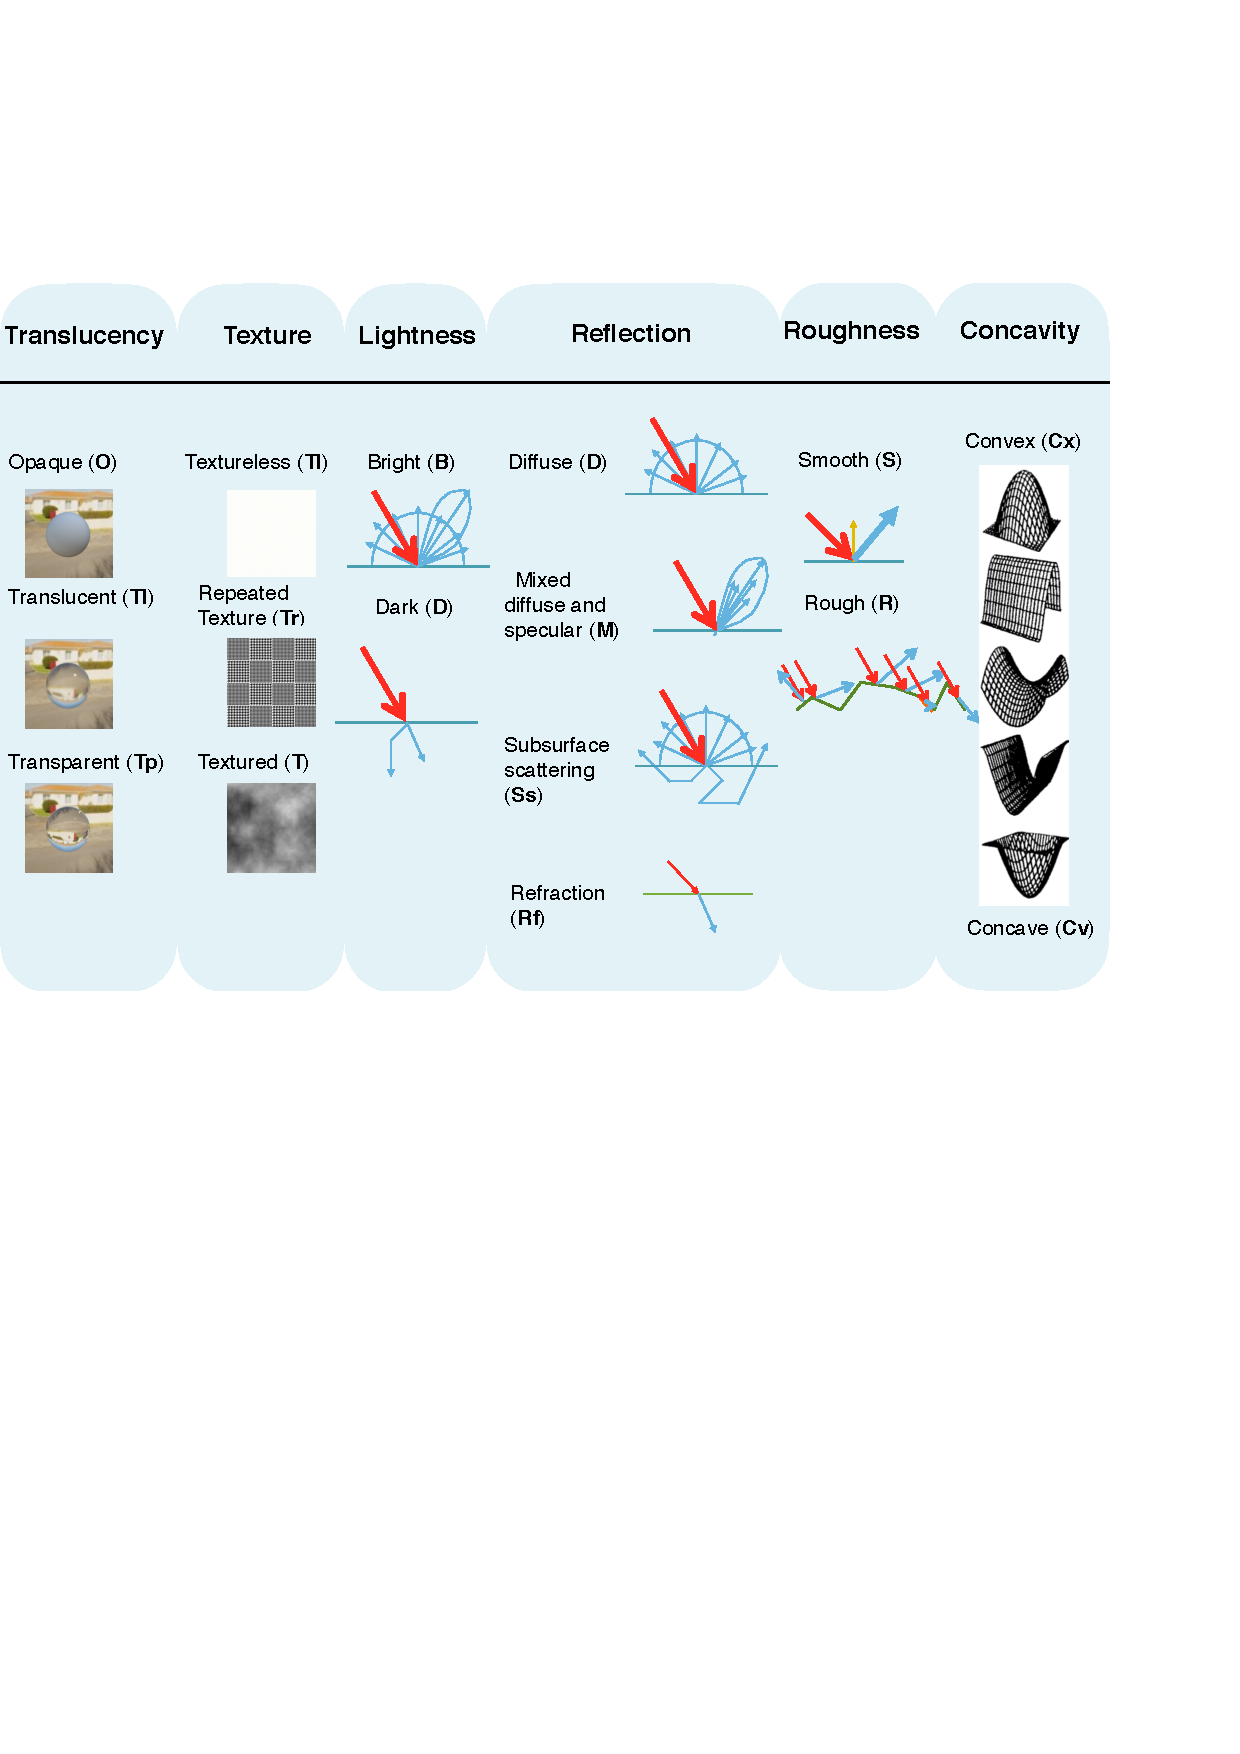
\includegraphics[width=0.7\textwidth]{prob_space/obj_class}
\end{figure}

\end{frame}

%------------------------------------------------
\begin{frame}{Problem space: four problem conditions}

\begin{exampleblock}{Assumptions}
\begin{table}
\centering
\begin{tabular}{ll}
\multirow{2}{*}{existence of algorithm} & translucency, transparency \\
& low surface reflectance (dark surfaces) \\ \cline{1-2}
\multirow{2}{*}{global interaction model} & transmission, refraction, inter-reflection \\
& severe concavity \\
\end{tabular}
\end{table}

\end{exampleblock}

\begin{figure}[h]
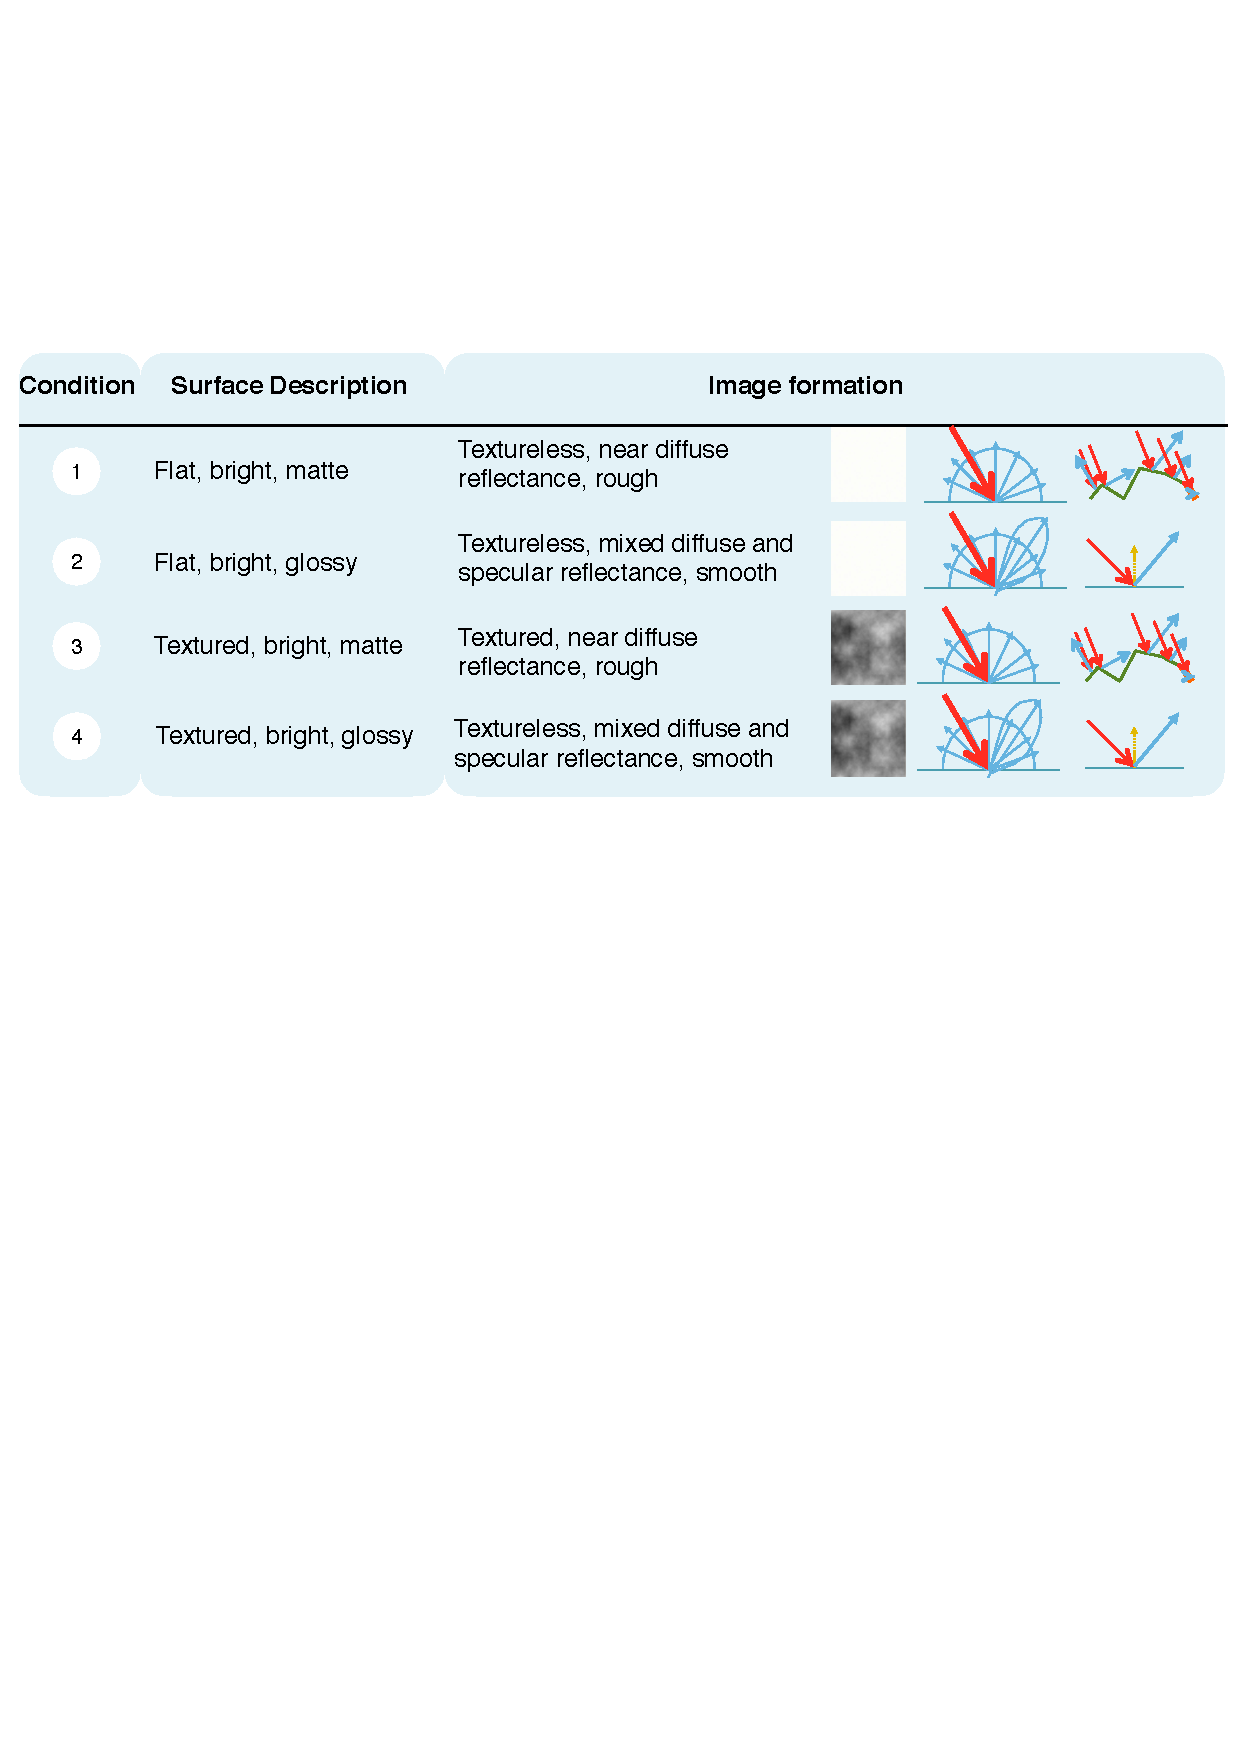
\includegraphics[width=0.7\textwidth]{prob_space/prob_cond}
\end{figure}

\end{frame}

%------------------------------------------------
\subsection{Description of 3D Reconstruction}
%------------------------------------------------
\begin{frame}{Description: model and representations}

\begin{table}
  \centering
  \begin{tabular}{lp{4cm}l}
  \textbf{Model} & \textbf{Representation} & \textbf{Example}\\ \cline{1-3}
  Nature of scene & \textit{Static} \\
  Lighting & \textit{Mixed: ambient, projector, light sources} \\
  Vantage point & \textit{Medium: 10 - 50} \\
  Texture & \textit{Texture randomness} & \raisebox{-.5\height}{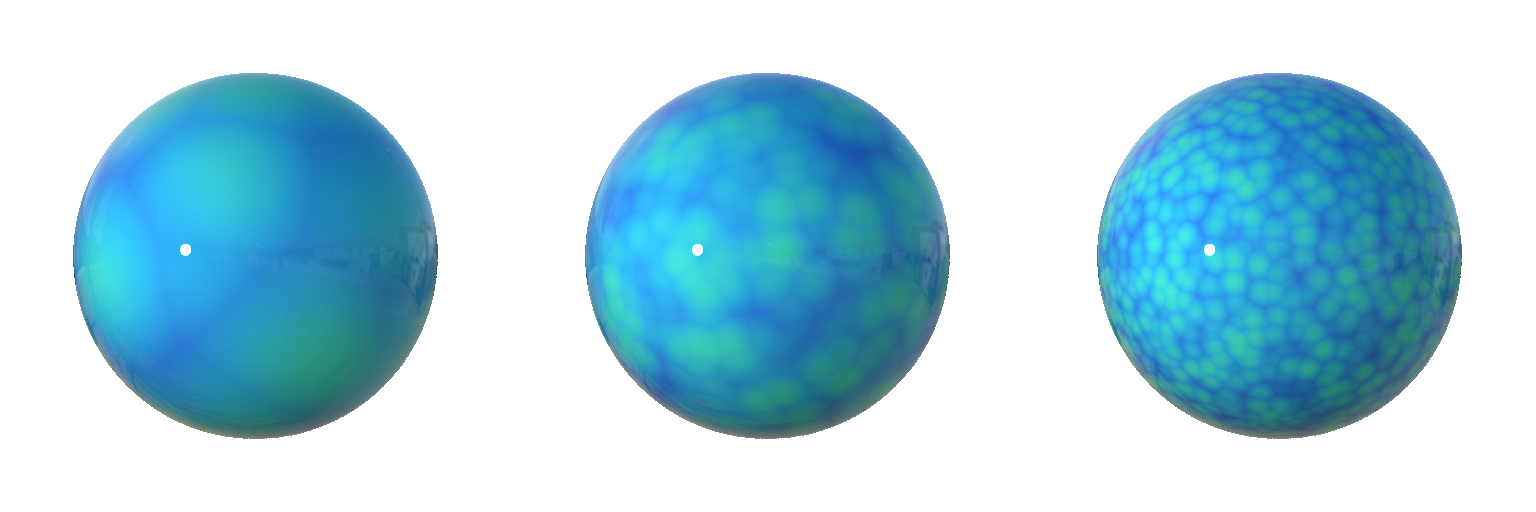
\includegraphics[width=0.3\textwidth]{mapping/setup/tex0}}\\
  Brightness & \textit{Diffuse reflectance} & \raisebox{-.5\height}{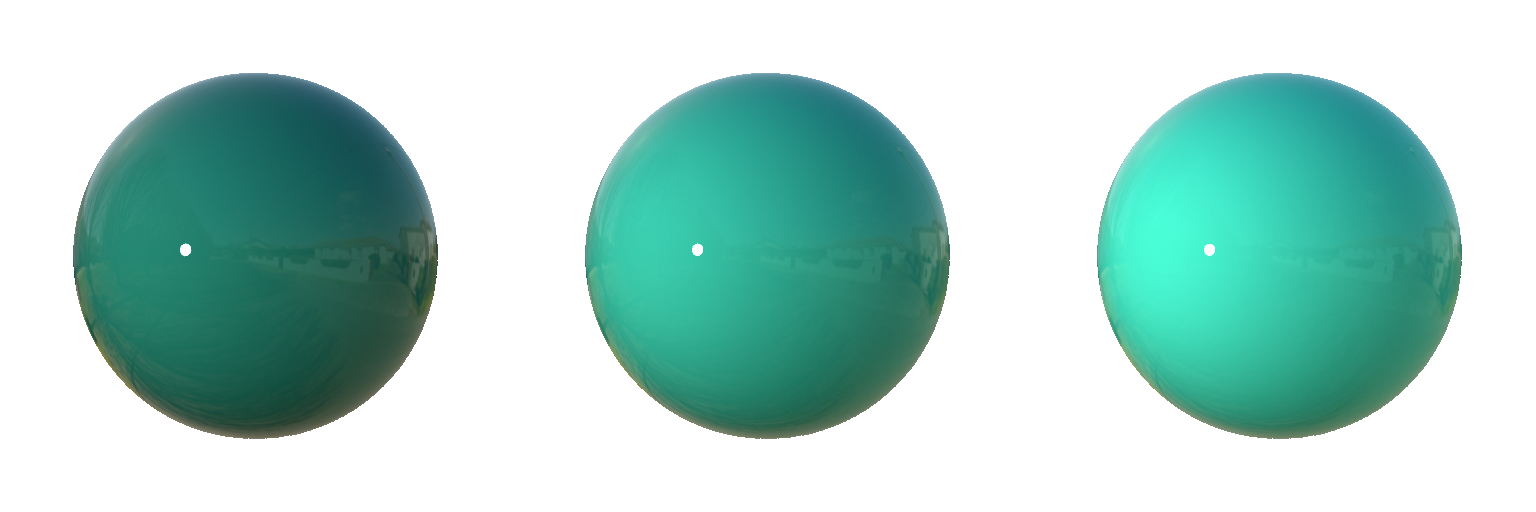
\includegraphics[width=0.3\textwidth]{mapping/setup/alb0}}\\
  Specularity & \textit{Fresnel reflectance} & \raisebox{-.5\height}{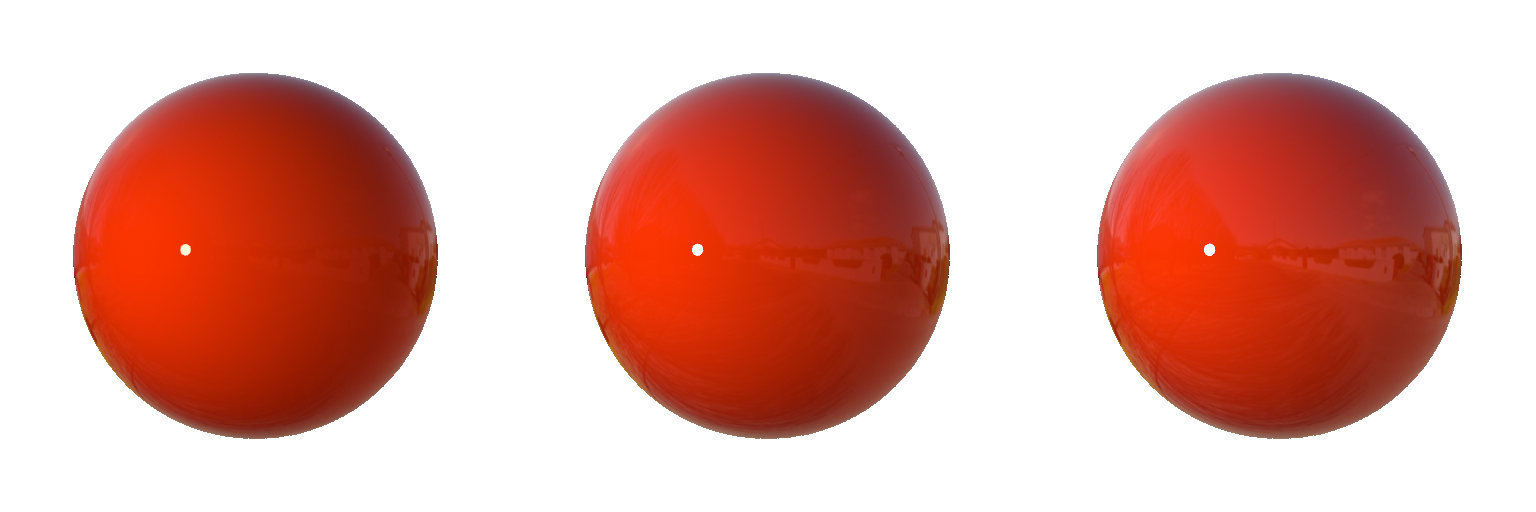
\includegraphics[width=0.3\textwidth]{mapping/setup/spec0}}\\
  Roughness & \textit{Distribution of facet normal} & \raisebox{-.5\height}{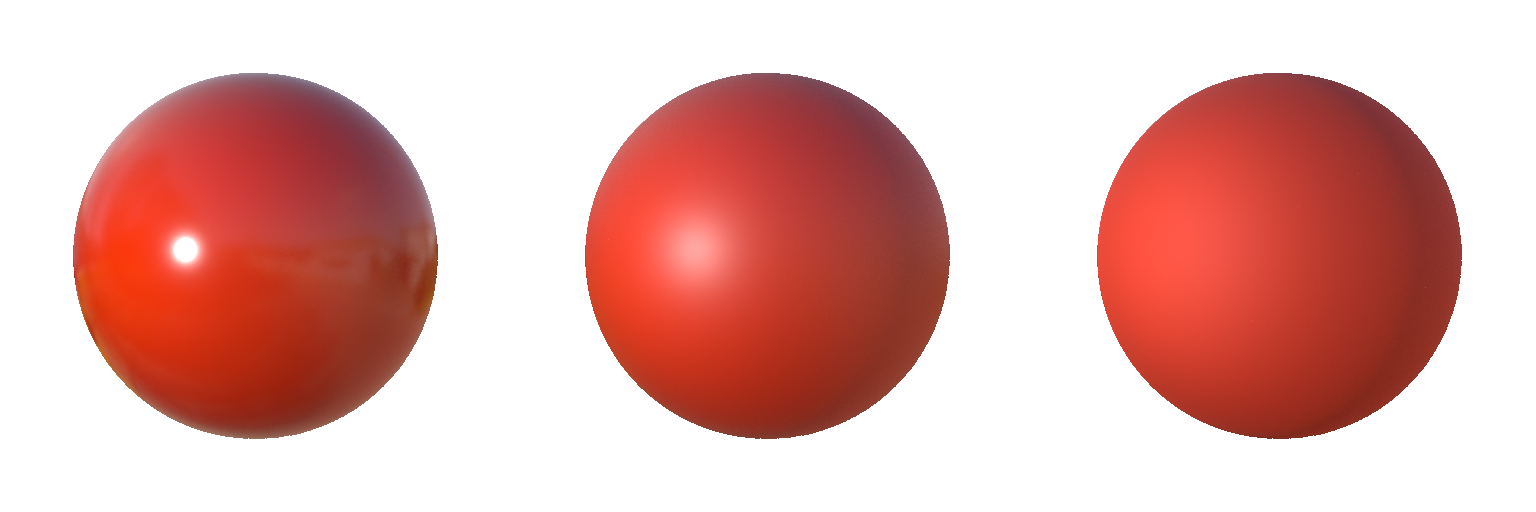
\includegraphics[width=0.3\textwidth]{mapping/setup/rough0}}\\
  % Concavity & \textit{Surface curvature}\\
  \end{tabular}
\end{table}

\end{frame}

%------------------------------------------------
\begin{frame}{Description: expression}

We use three-scale values to parameterize properties: \textit{low} (0.2), \textit{medium} (0.5), and \textit{high} (0.8).

\begin{figure}[!htbp]
\centering
\begin{tabular}{cccc}
  \includegraphics[width=0.25\textwidth]{images/desc_vase.pdf}&
  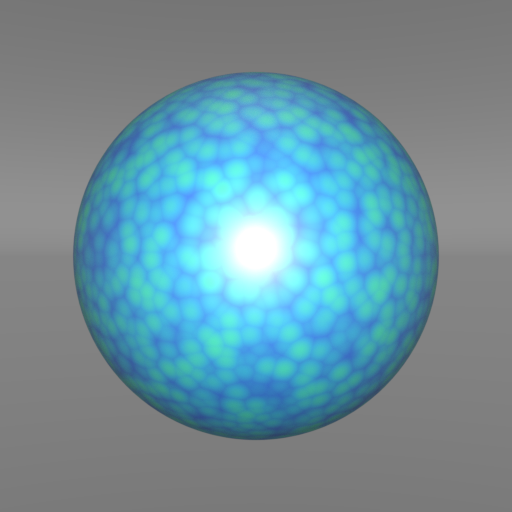
\includegraphics[width=0.2\textwidth]{interp/ui/ui_sphere.png}&
  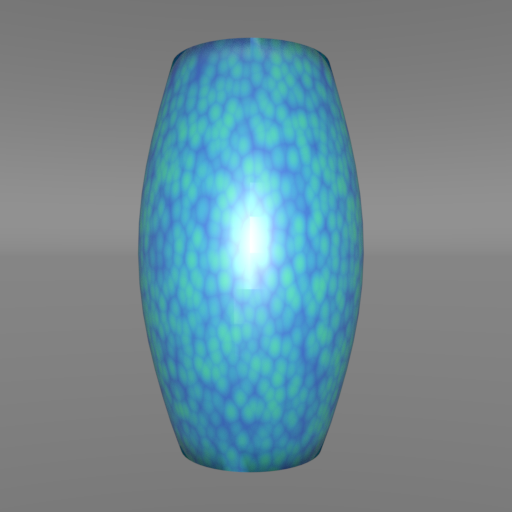
\includegraphics[width=0.2\textwidth]{interp/ui/ui_vase.png}&
  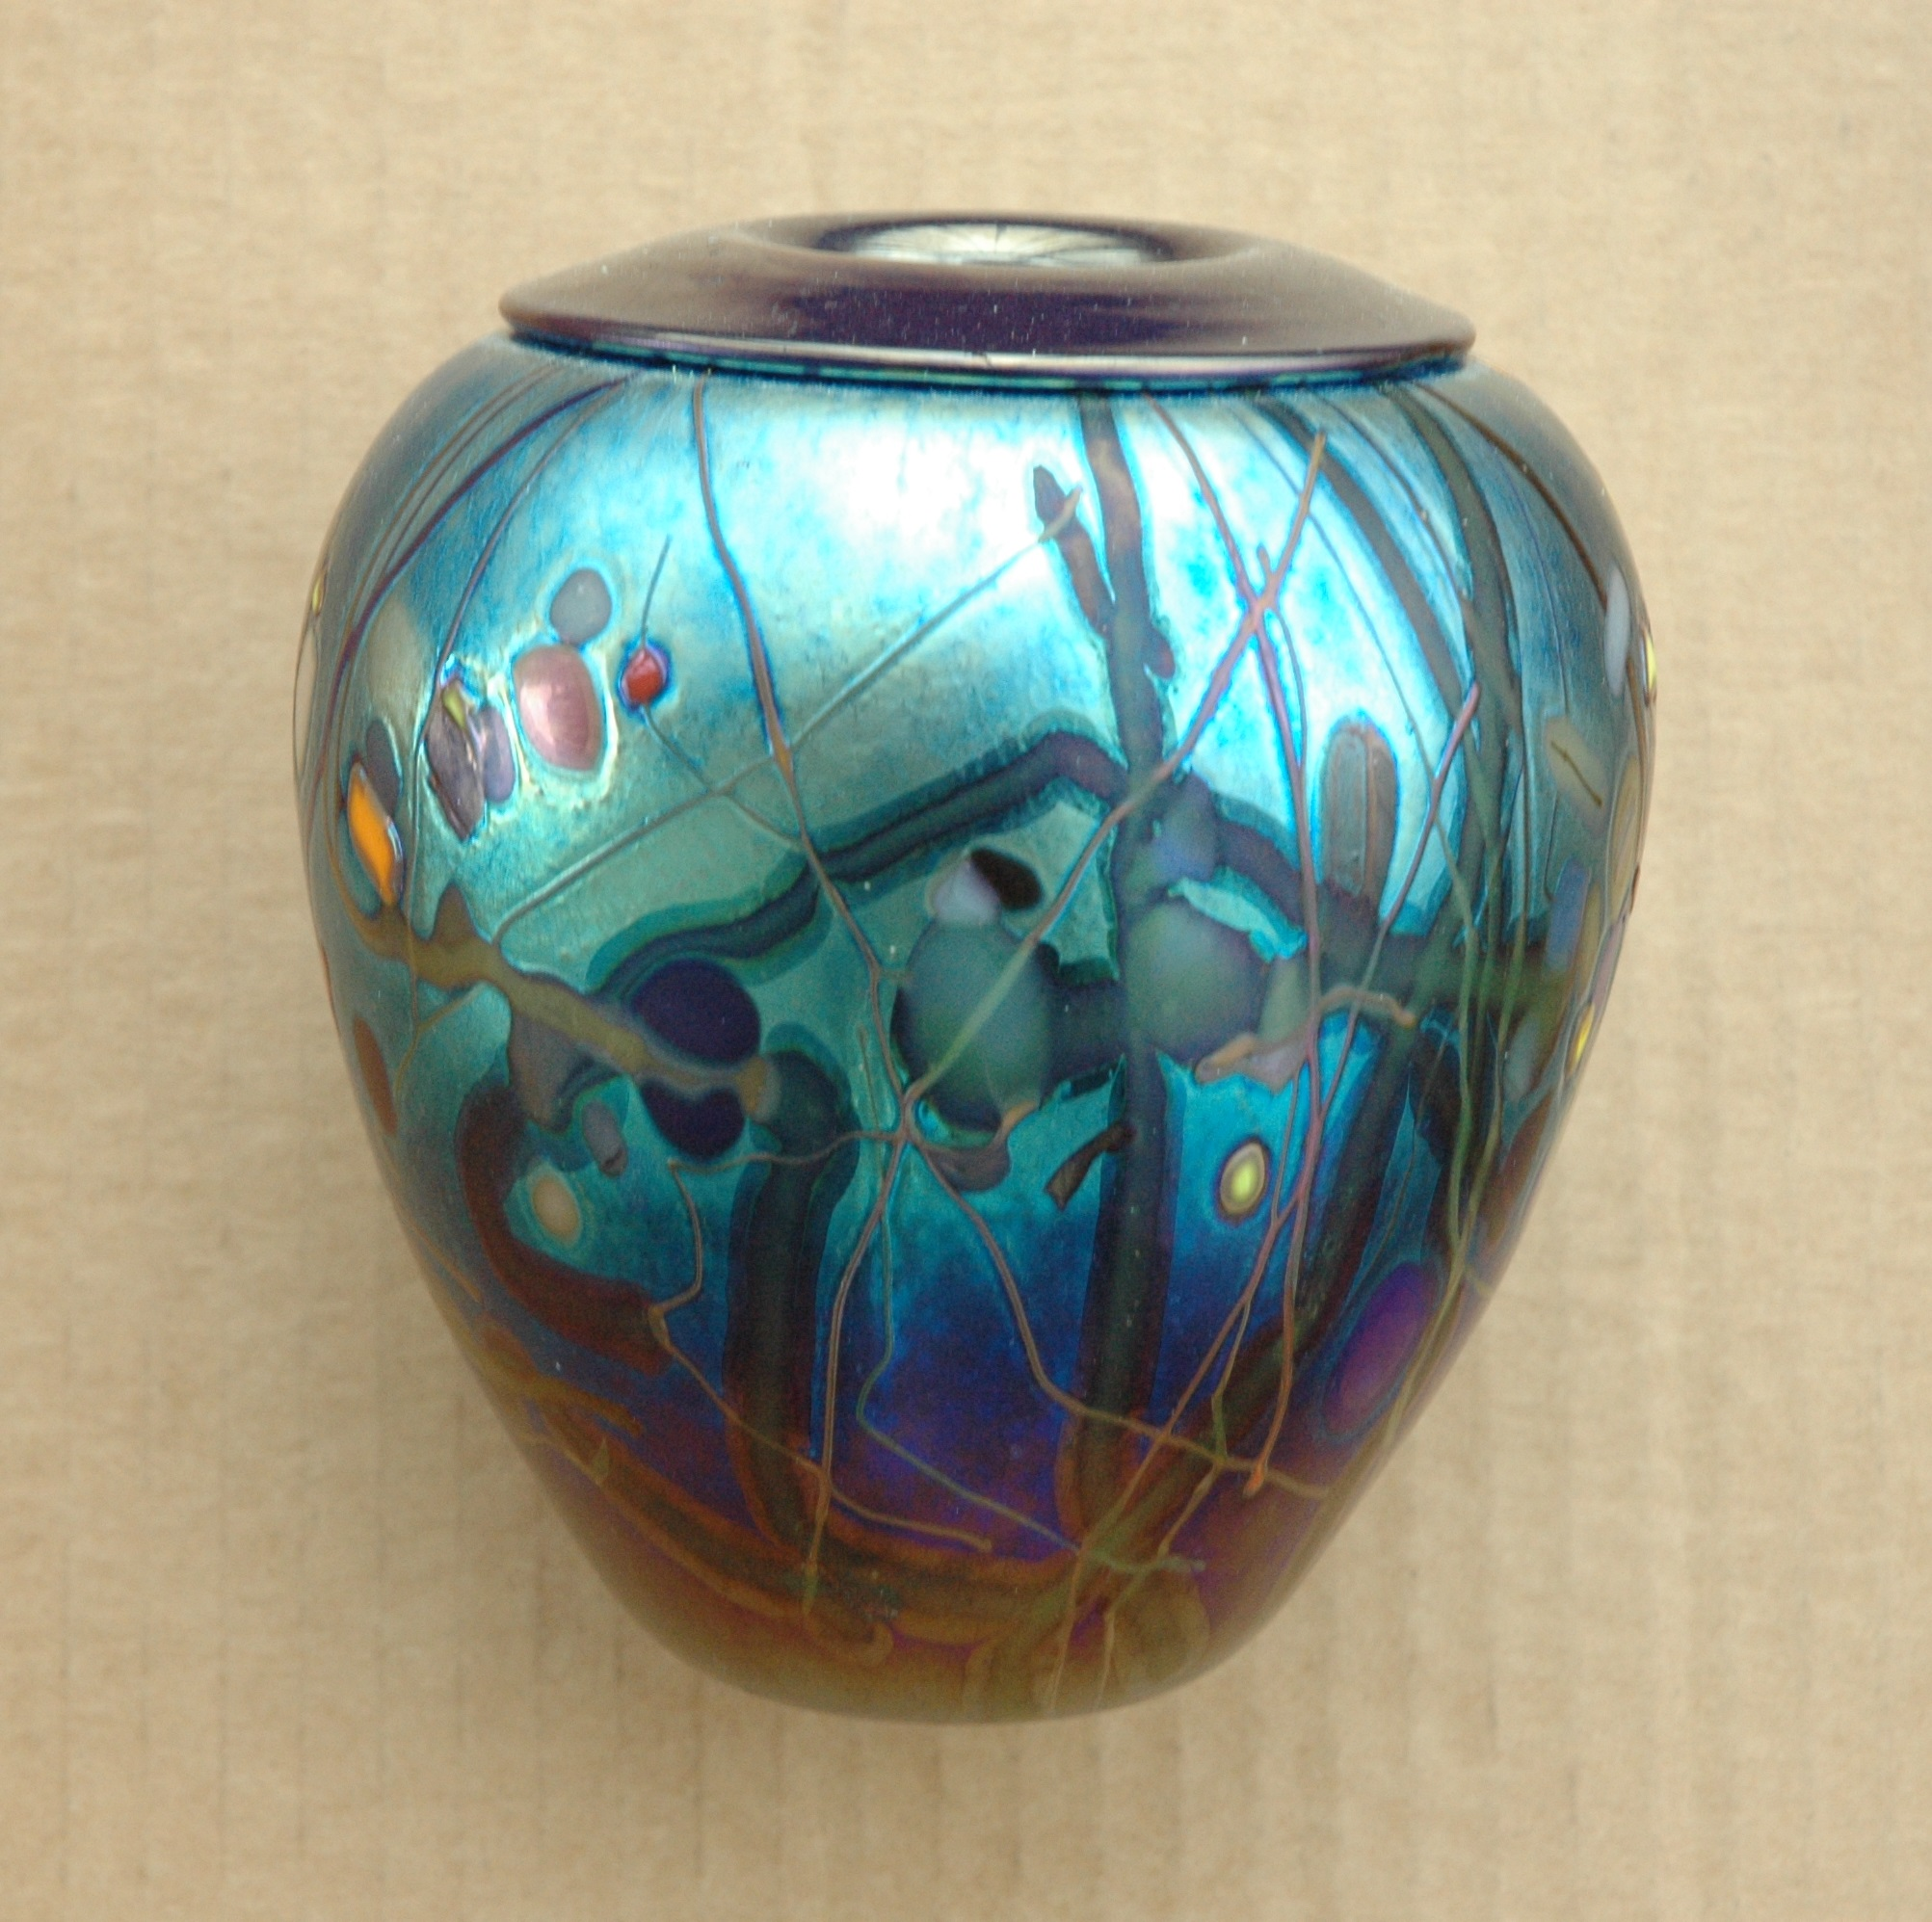
\includegraphics[width=0.2\textwidth]{interp/real_world_img/vase/vase.jpg}\\
  Property settings & Synthetic sphere & Synthetic vase & Real-world vase\\
\end{tabular}
% \caption{(a) demonstrates the effect of the property settings on a sphere, (b) on a teapot, and (c) shows the real-world object.}
\end{figure}

\end{frame}

%------------------------------------------------
\subsection{Mapping of 3D Reconstruction}
%------------------------------------------------
\begin{frame}{Mapping}

% Investigate the problem conditions under which the algorithms can reliably work.

\begin{figure}
\centering
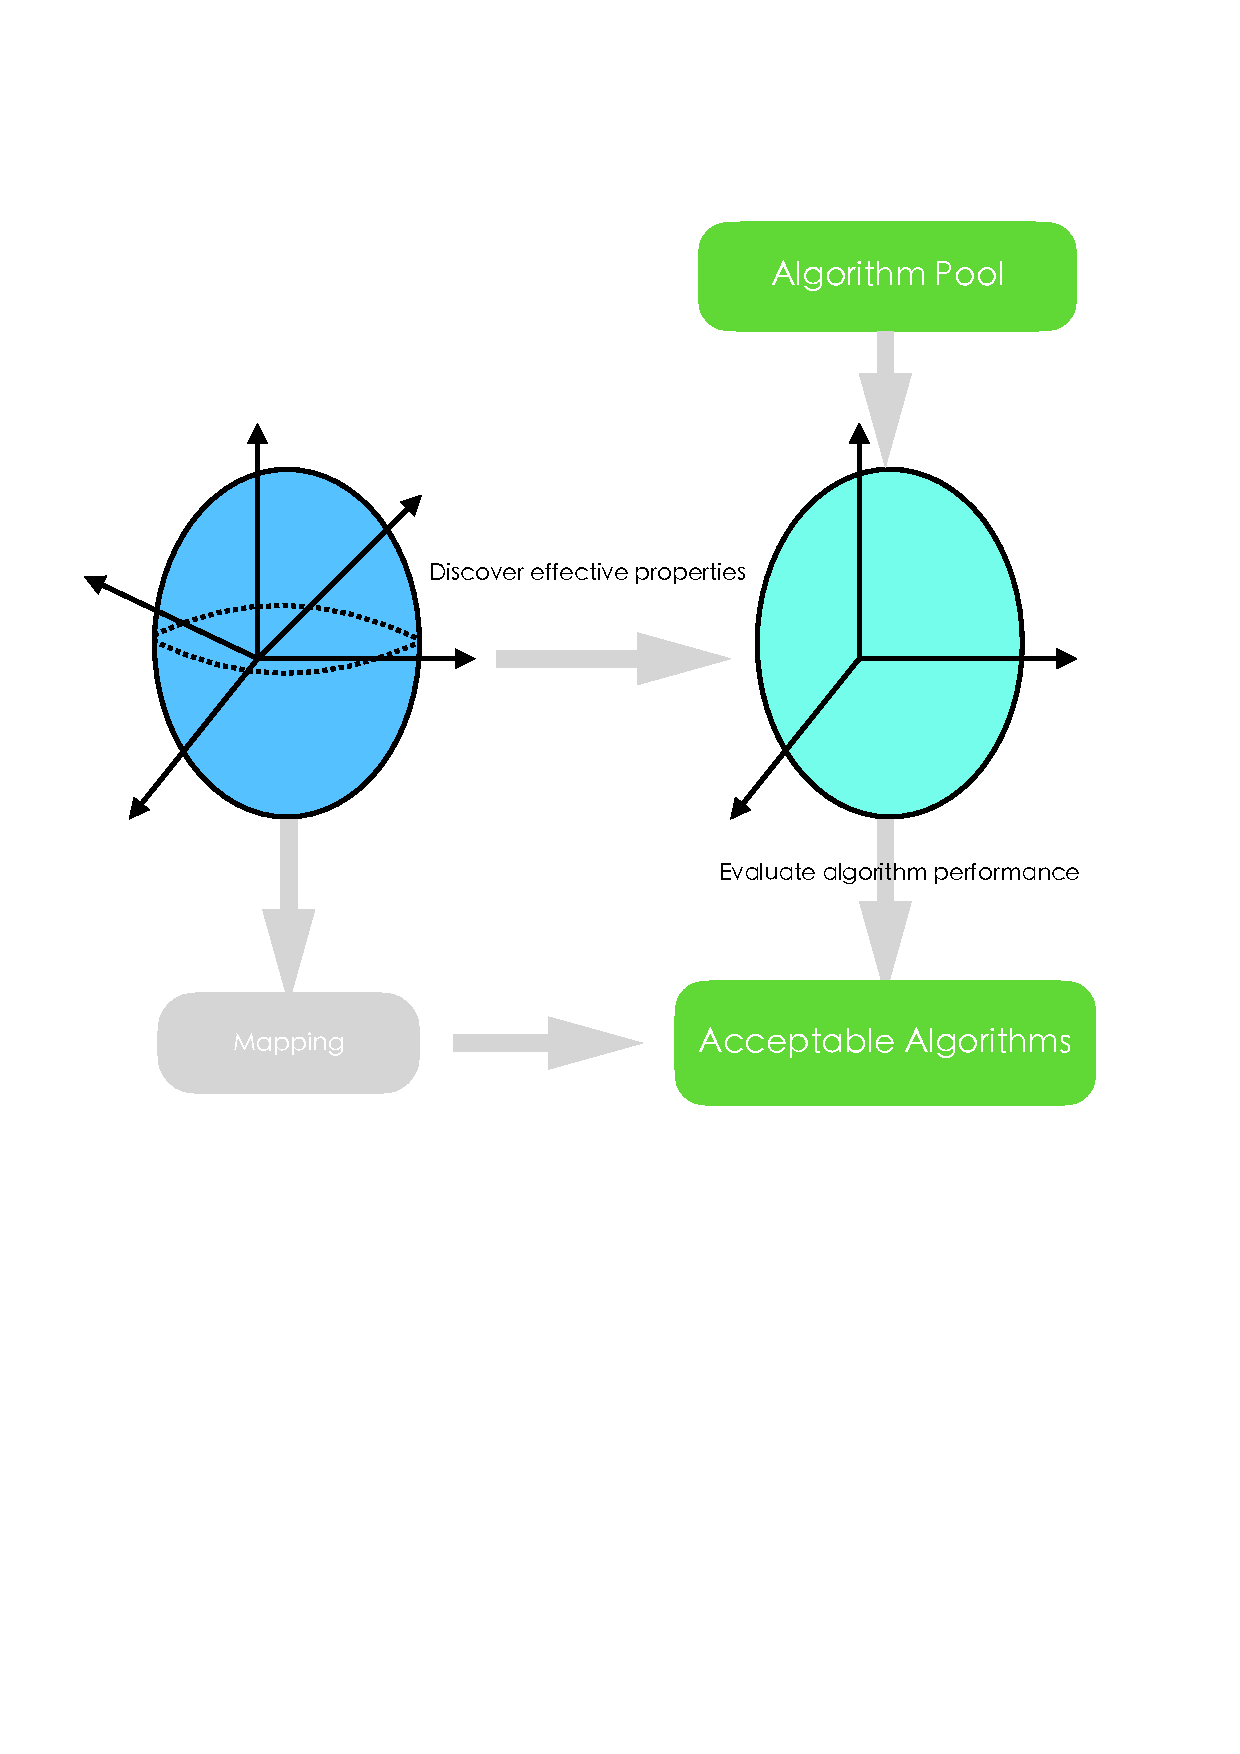
\includegraphics[width=0.9\textwidth]{images/mapping_3d_vision.pdf}
\end{figure}

% \begin{itemize}
% \item Establish the \textit{effective problem domain} (EPD): cope with large variation in material and shape.
% \item Evaluate algorithmic performance within EPD
% \item Derive mapping from problem conditions to algorithms.
% \end{itemize}

\end{frame}

%------------------------------------------------
\begin{frame}{Mapping: algorithms}

\begin{exampleblock}{selected algorithms}
\begin{itemize}
\item Patch-based Multi-View Stereo (PMVS): propagate-refinement-filtering;
\item Example-based Photometric Stereo (EPS): arbitrary BRDF is a linear combination of basis BRDFs;
\item Gray-coded Structured Light (GSL): encode spatial informally temporally.
\end{itemize}
\end{exampleblock}

\begin{exampleblock}{baseline methods}
\begin{itemize}
\item Volumetric Visual Hull: carve voxels projecting outside of silhouettes;
\item Linear-least squares Photometric Stereo: $\mathbf{I}=\rho\mathbf{N}\cdot\mathbf{L}$
\end{itemize}
\end{exampleblock}

\end{frame}

%------------------------------------------------
\begin{frame}{Mapping: reduce dimensionality}

Reduce problem space dimensionality by discovering properties that have an effect on algorithm performance.
\begin{figure}
\centering
\includegraphics[width=0.5\textwidth]{mapping/eval_prop/mvs_tex_spec}
\end{figure}

\begin{exampleblock}{observations}
\begin{itemize}
\item texture and specularity has an effect on both accuracy and completeness;
\item the effect of specularity is less noticable on highly/lowly textured surfaces.
\end{itemize}
\end{exampleblock}

\end{frame}

%------------------------------------------------
\begin{frame}{Mapping: discover mapping}

Discover the mapping from problem condition to algorithms
\begin{figure}
\centering
\includegraphics[width=0.5\textwidth]{mapping/lookup_table/mvs_texture_05}
\end{figure}

\begin{table}
\centering
\begin{tabular}{*{4}{c}}
\toprule
Texture & Albedo & Specular & Roughness\\
\midrule
0.5 & 0.5 & 0.2 & -\\
0.5 & 0.8 & 0.2 & -\\
0.5 & 0.8 & 0.5 & -\\
\bottomrule
\end{tabular}
\caption{Problem conditions that PMVS works reliably under.}
\end{table}

\end{frame}

%------------------------------------------------
\section{Application of Interface}
%------------------------------------------------
\begin{frame}{Interpretation: evaluation methodology}

\begin{exampleblock}{Evaluation questions}
  1. accurate description $\Rightarrow$ successful result; \\
  2. less accurate description $\Rightarrow$ less successful result;\\
  3. inaccurate description $\Rightarrow$ poor result; \\
\end{exampleblock}

\begin{exampleblock}{Criteria}
  Visual comparison.
\end{exampleblock}

\begin{figure}
\centering
\begin{tabular}{ccc}
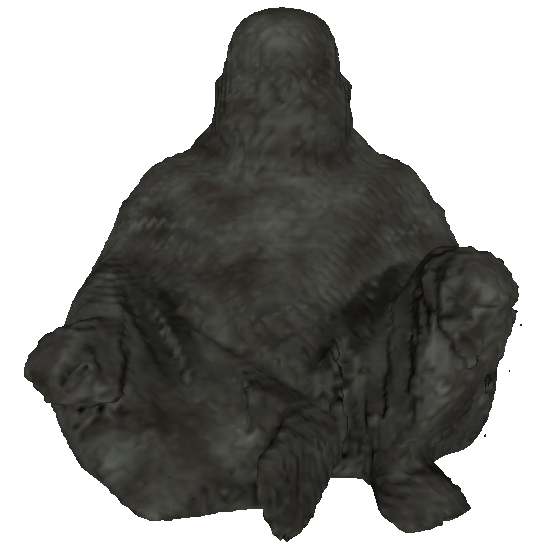
\includegraphics[width=0.2\textwidth]{interp/synth_interp/budda_vh} &
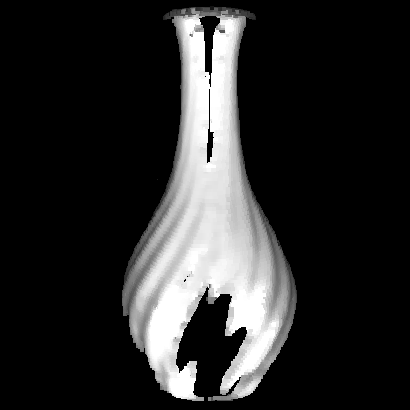
\includegraphics[width=0.2\textwidth]{interp/synth_interp/vase0_sl} &
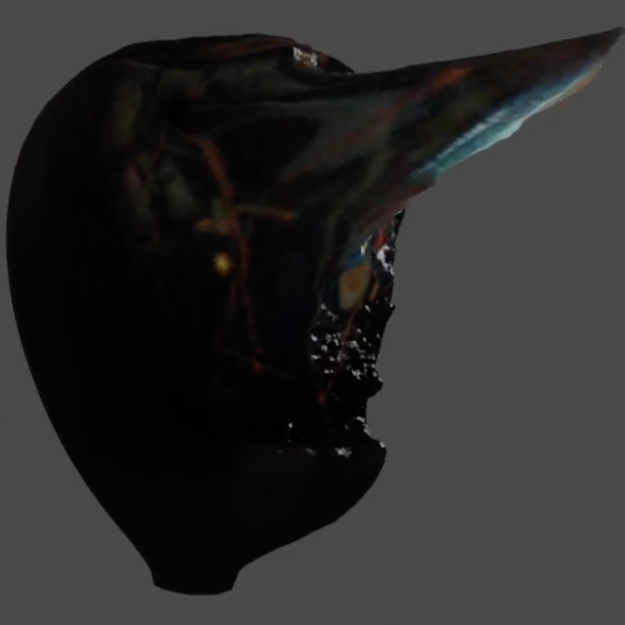
\includegraphics[width=0.2\textwidth]{interp/real_interp/vase/vase_spike} \\
accuracy & completenss & angle diff \\
\end{tabular}
\end{figure}

\end{frame}

%------------------------------------------------
% \begin{frame}{Interpretation: evaluation methodology (cont'd)}

% \begin{exampleblock}{Roadmap}
%   \begin{itemize}
%     \item proof of concept interpreter;
%     \item dataset creation;
%     \item results of interpreter.
%   \end{itemize}
% \end{exampleblock}

% \end{frame}

%------------------------------------------------
\begin{frame}{Interpretation: proof of concept interpreter}

Interpreter: selects an algorithm based on a description.

\begin{figure}[!htbp]
\centering
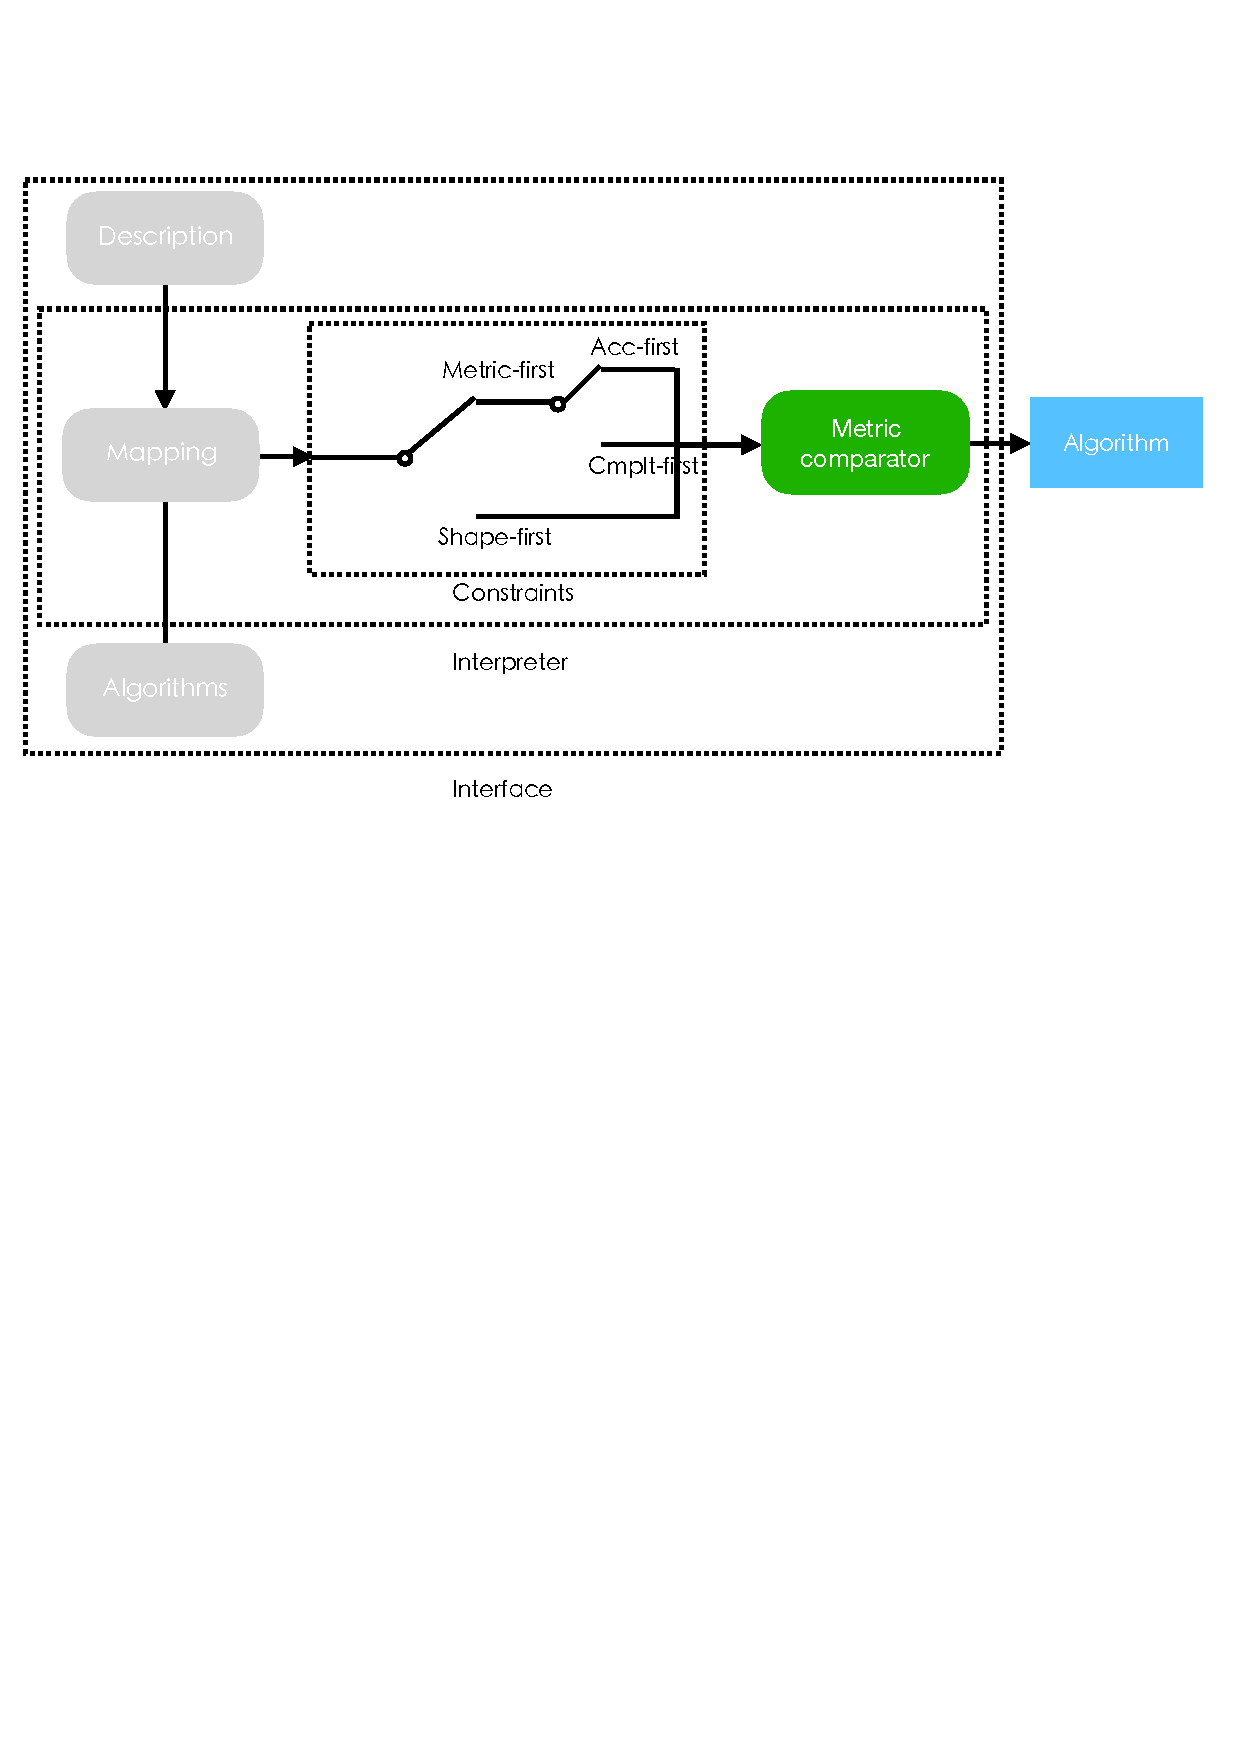
\includegraphics[width=0.7\textwidth]{interp/interpreter.pdf}
\end{figure}

\end{frame}

%------------------------------------------------
% \begin{frame}{Interpretation: dataset creation}

% \begin{exampleblock}{Setup}
%   \begin{table}
%     \begin{tabular}{l|l|l}
%     method & hardware & configuration \\
%     \midrule
%     MVS+VH & camera & 3 heights, $30^\circ$ baseline angle \\
%     PS & camera, lamp, 2 ref objs & \\
%     SL & camera, projector & $10^\circ$ baseline angle\\
%     \end{tabular}
%   \end{table}
% \end{exampleblock}

% \begin{exampleblock}{Calibration}
%   \begin{table}
%     \begin{tabular}{l|l}
%     method & calibration \\
%     \midrule
%     MVS+VH & focal length from EXIF, extrinsics using SfM \\
%     PS & no radiometric calibration performed \\
%     SL & camera-projector calibration using local homography \\
%     \end{tabular}
%   \end{table}
% \end{exampleblock}

% \end{frame}

%------------------------------------------------
\begin{frame}{Interpretation: dataset}

Objects meet the requirements of the four problem conditions.

\begin{figure}[!htbp]
\centering
\begin{tabular}{p{0.6cm}*{4}{p{1.5cm}}}
Cond & 1 & 2 & 3 & 4\\
\midrule
\multirow{2}{*}{\rotatebox[origin=c]{90}{object}} & 
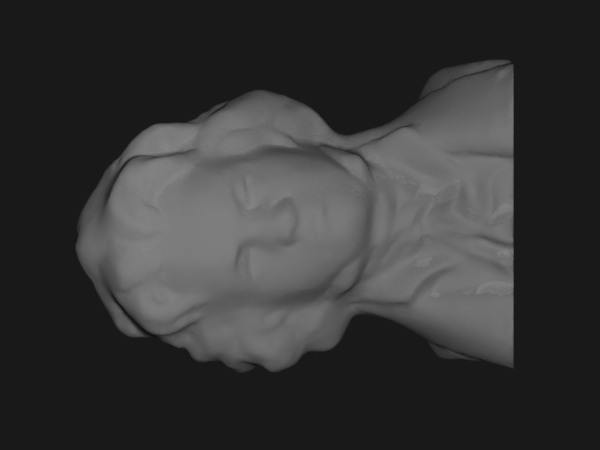
\includegraphics[width=0.15\textwidth]{interp/synth_data/bust} &
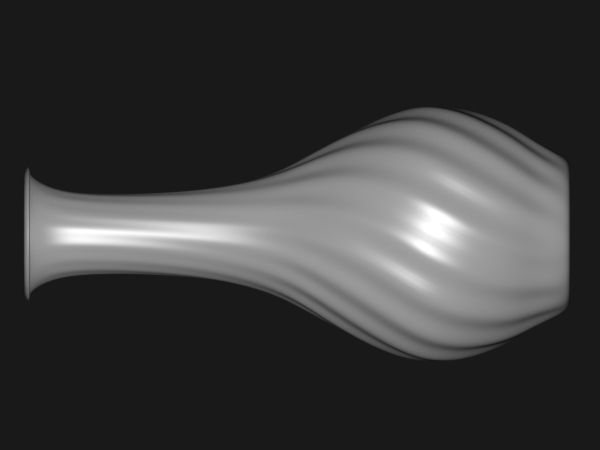
\includegraphics[width=0.15\textwidth]{interp/synth_data/vase0} &
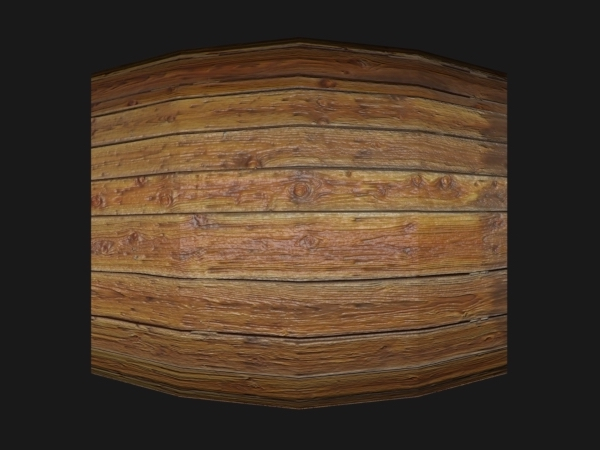
\includegraphics[width=0.15\textwidth]{interp/synth_data/barrel} &
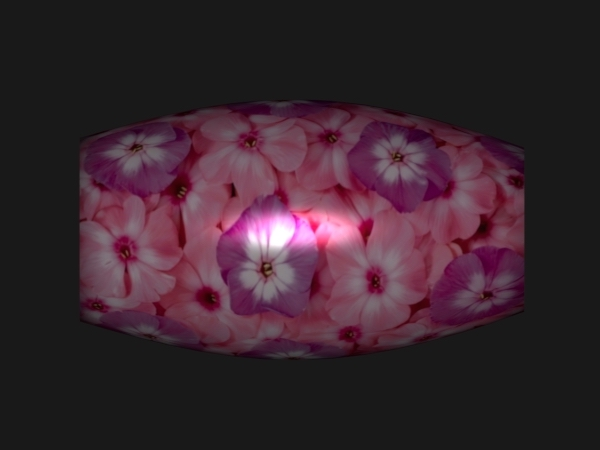
\includegraphics[width=0.15\textwidth]{interp/synth_data/vase1}\\
& 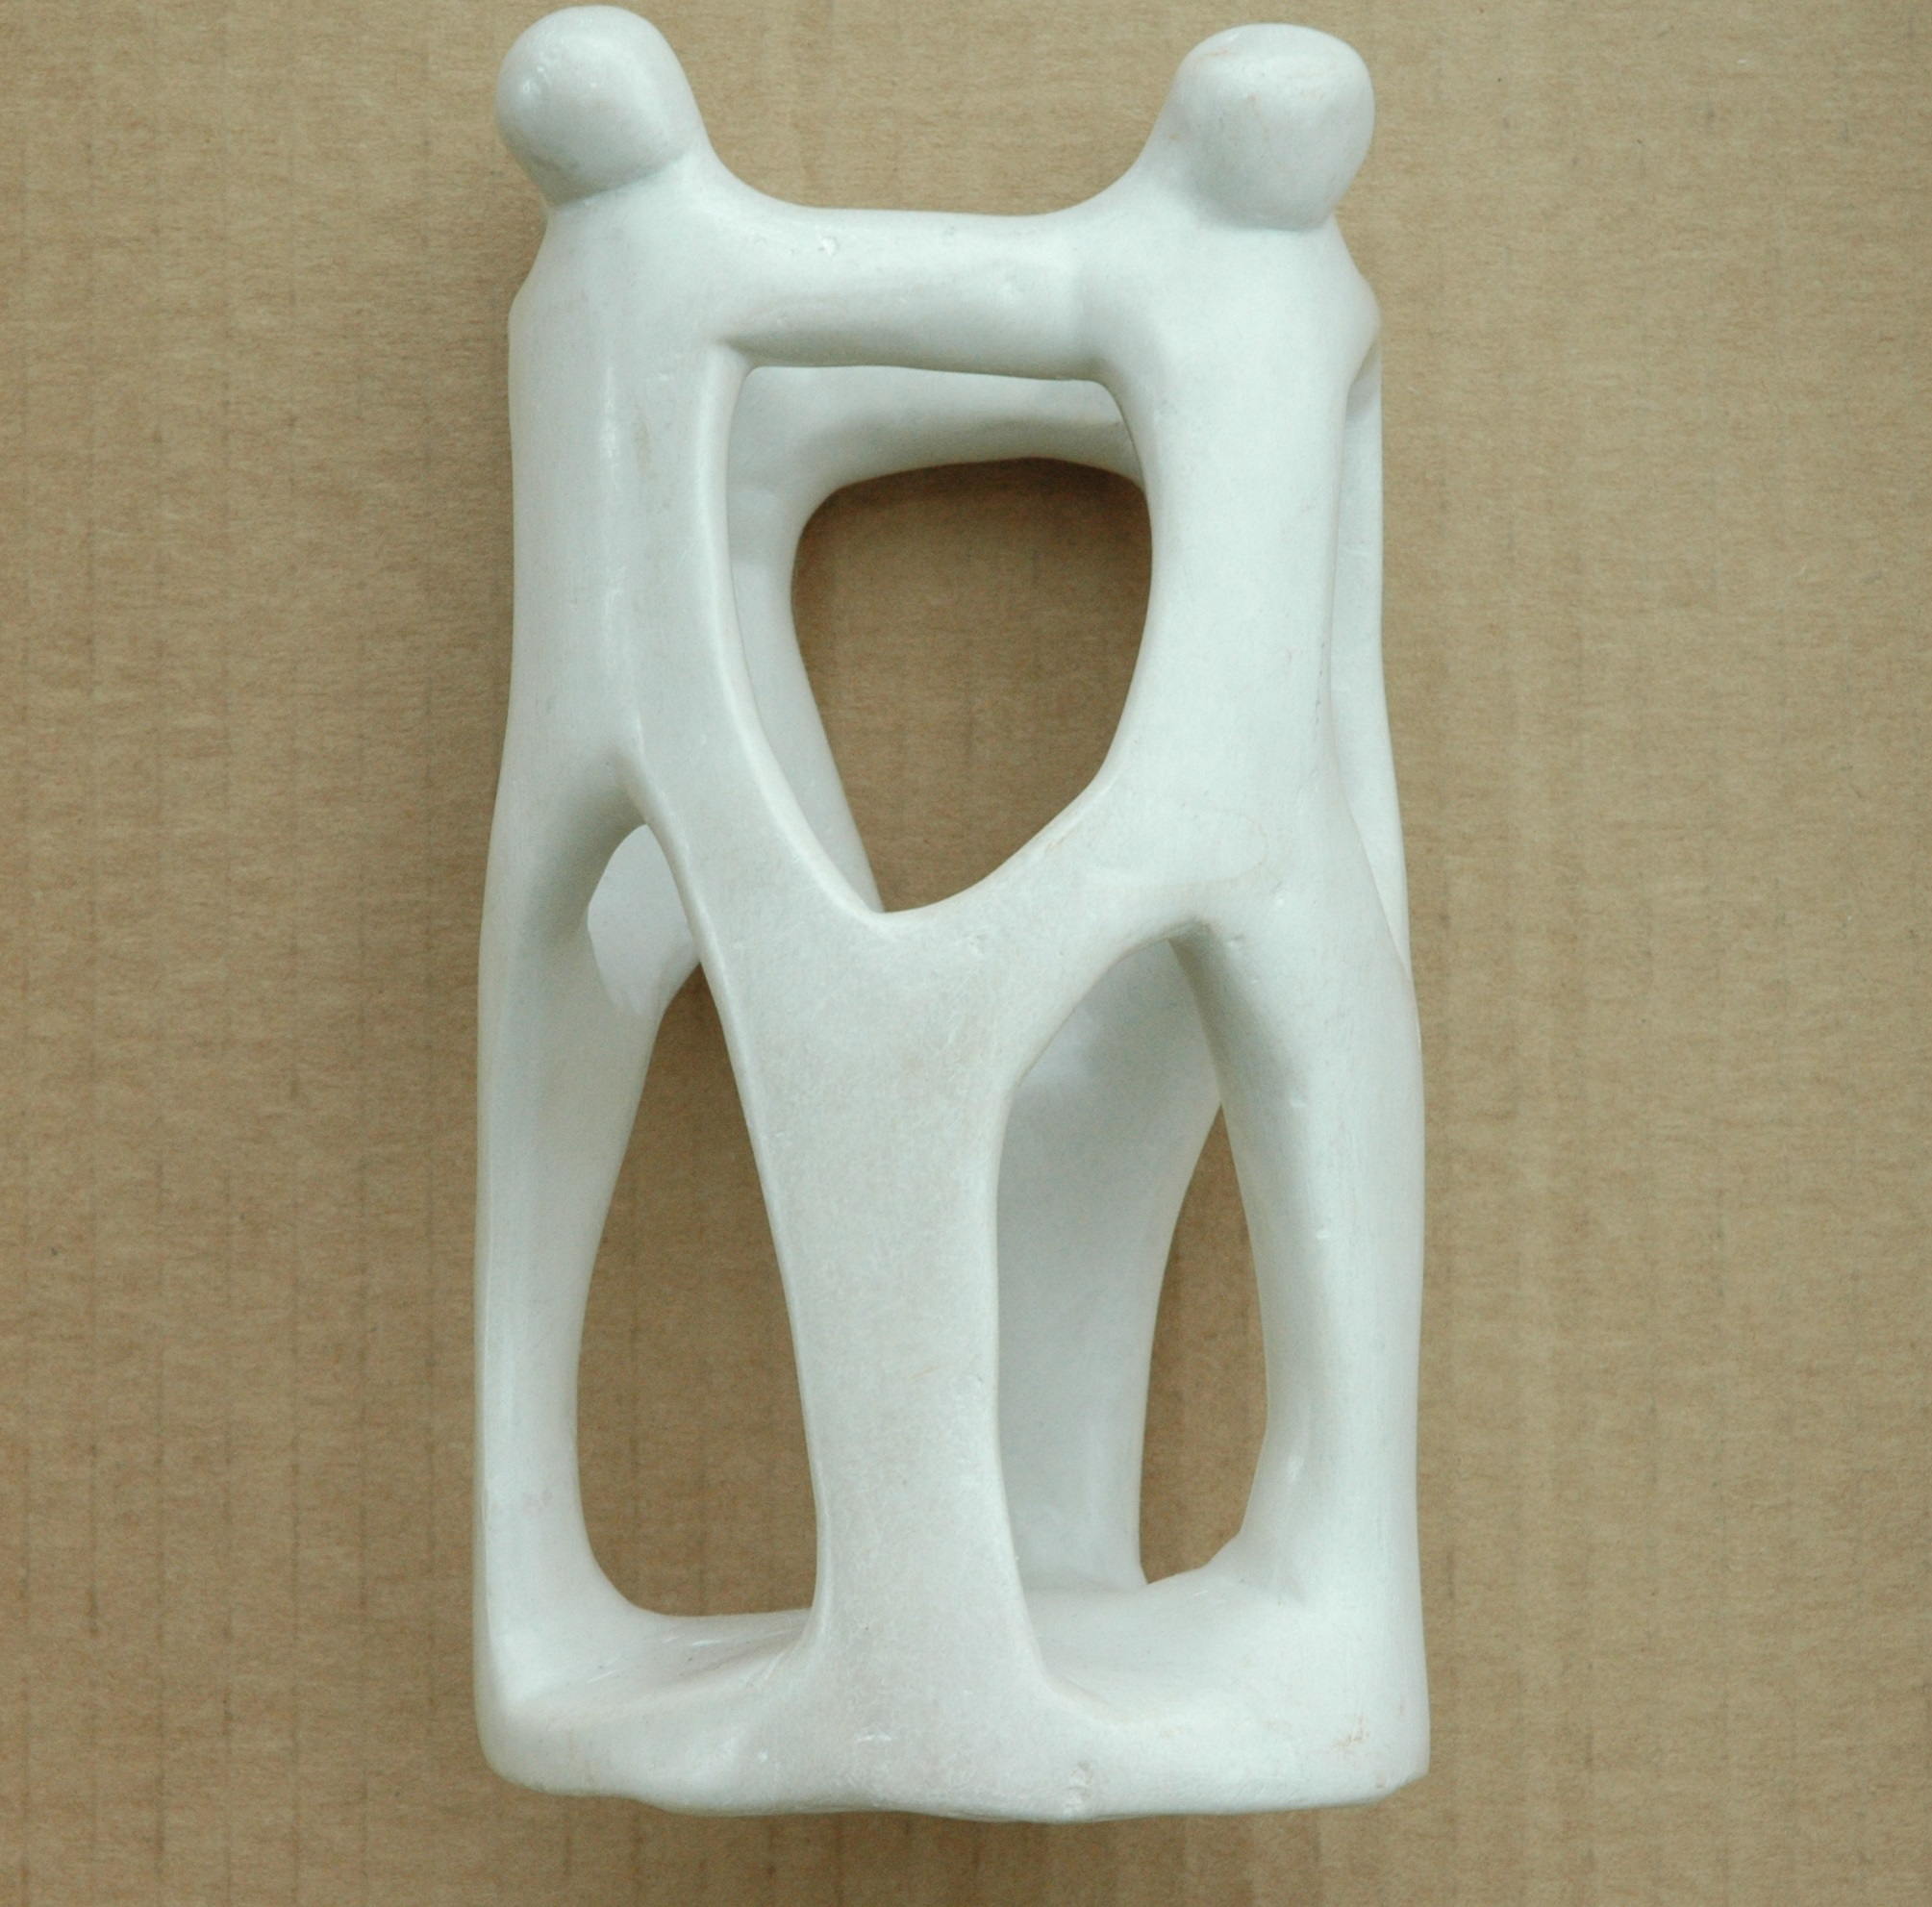
\includegraphics[width=0.15\textwidth]{interp/real_world_img/statue/statue} &
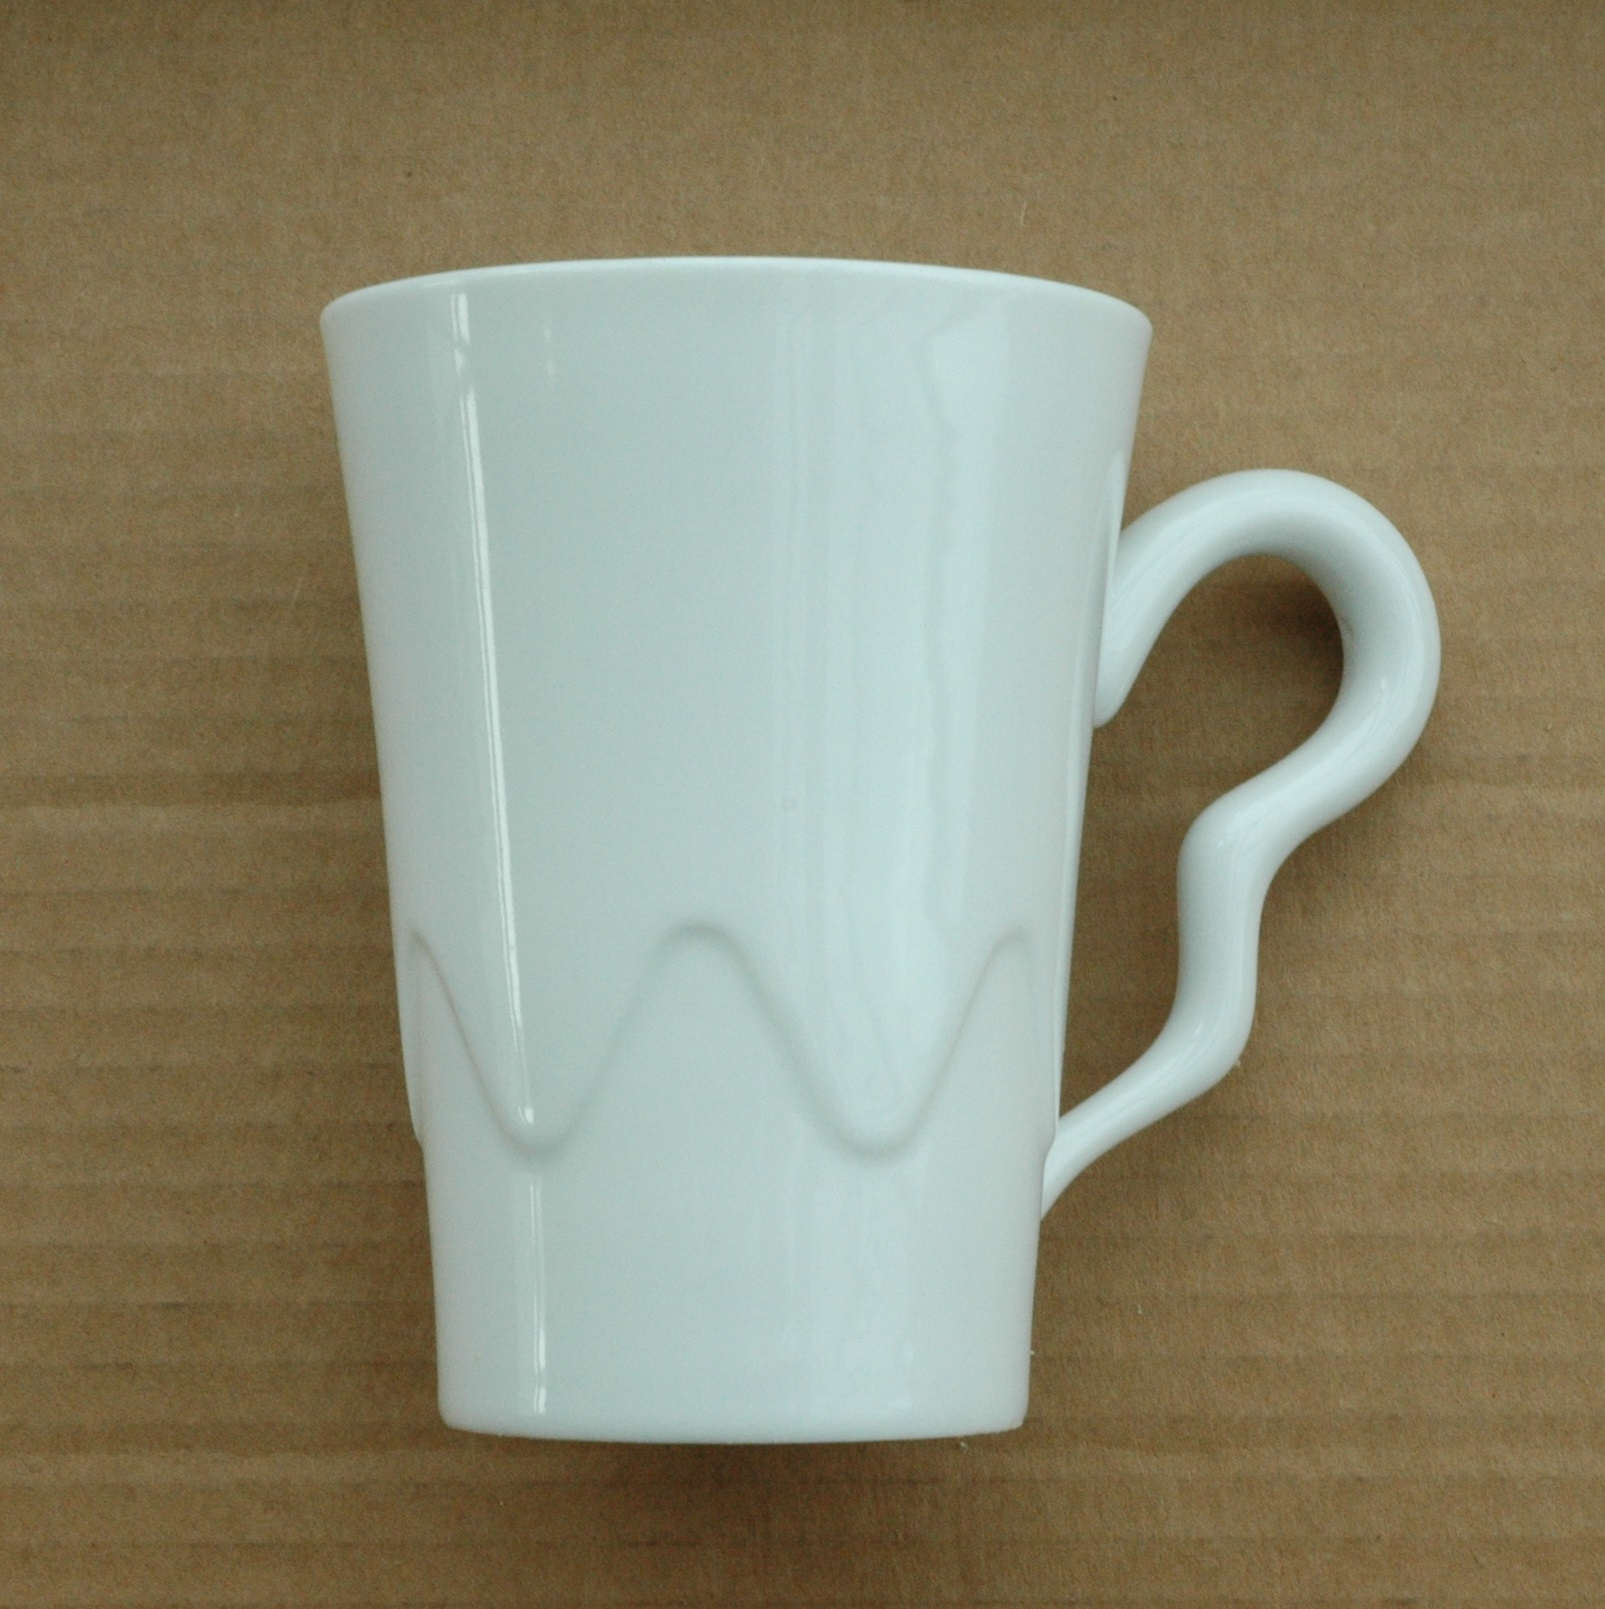
\includegraphics[width=0.15\textwidth]{interp/real_world_img/cup/cup} &
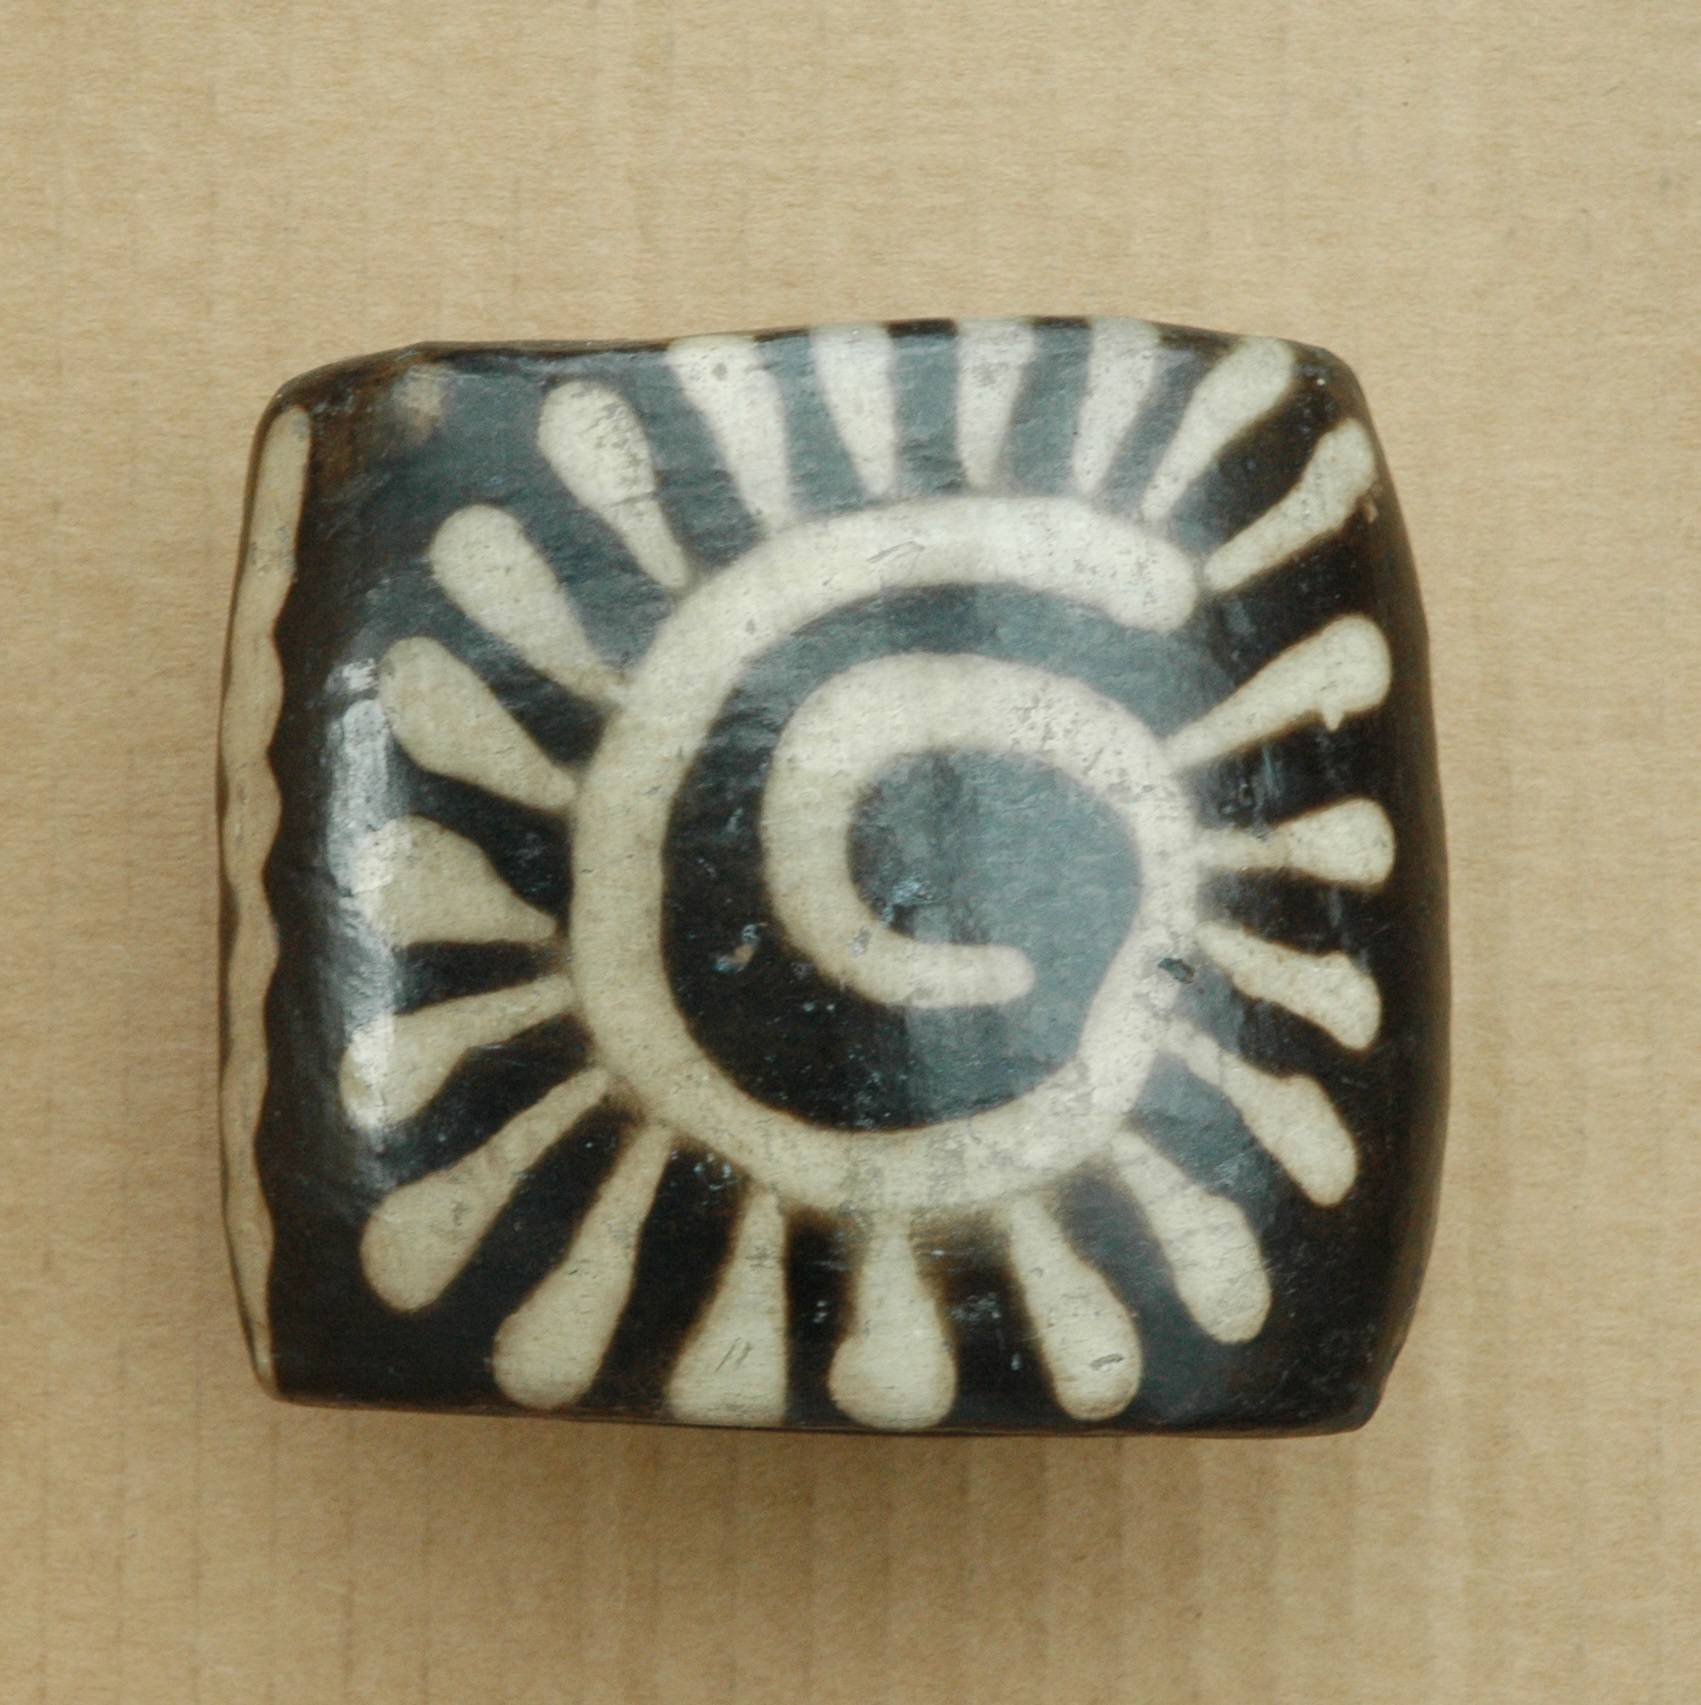
\includegraphics[width=0.15\textwidth]{interp/real_world_img/pot/pot} &
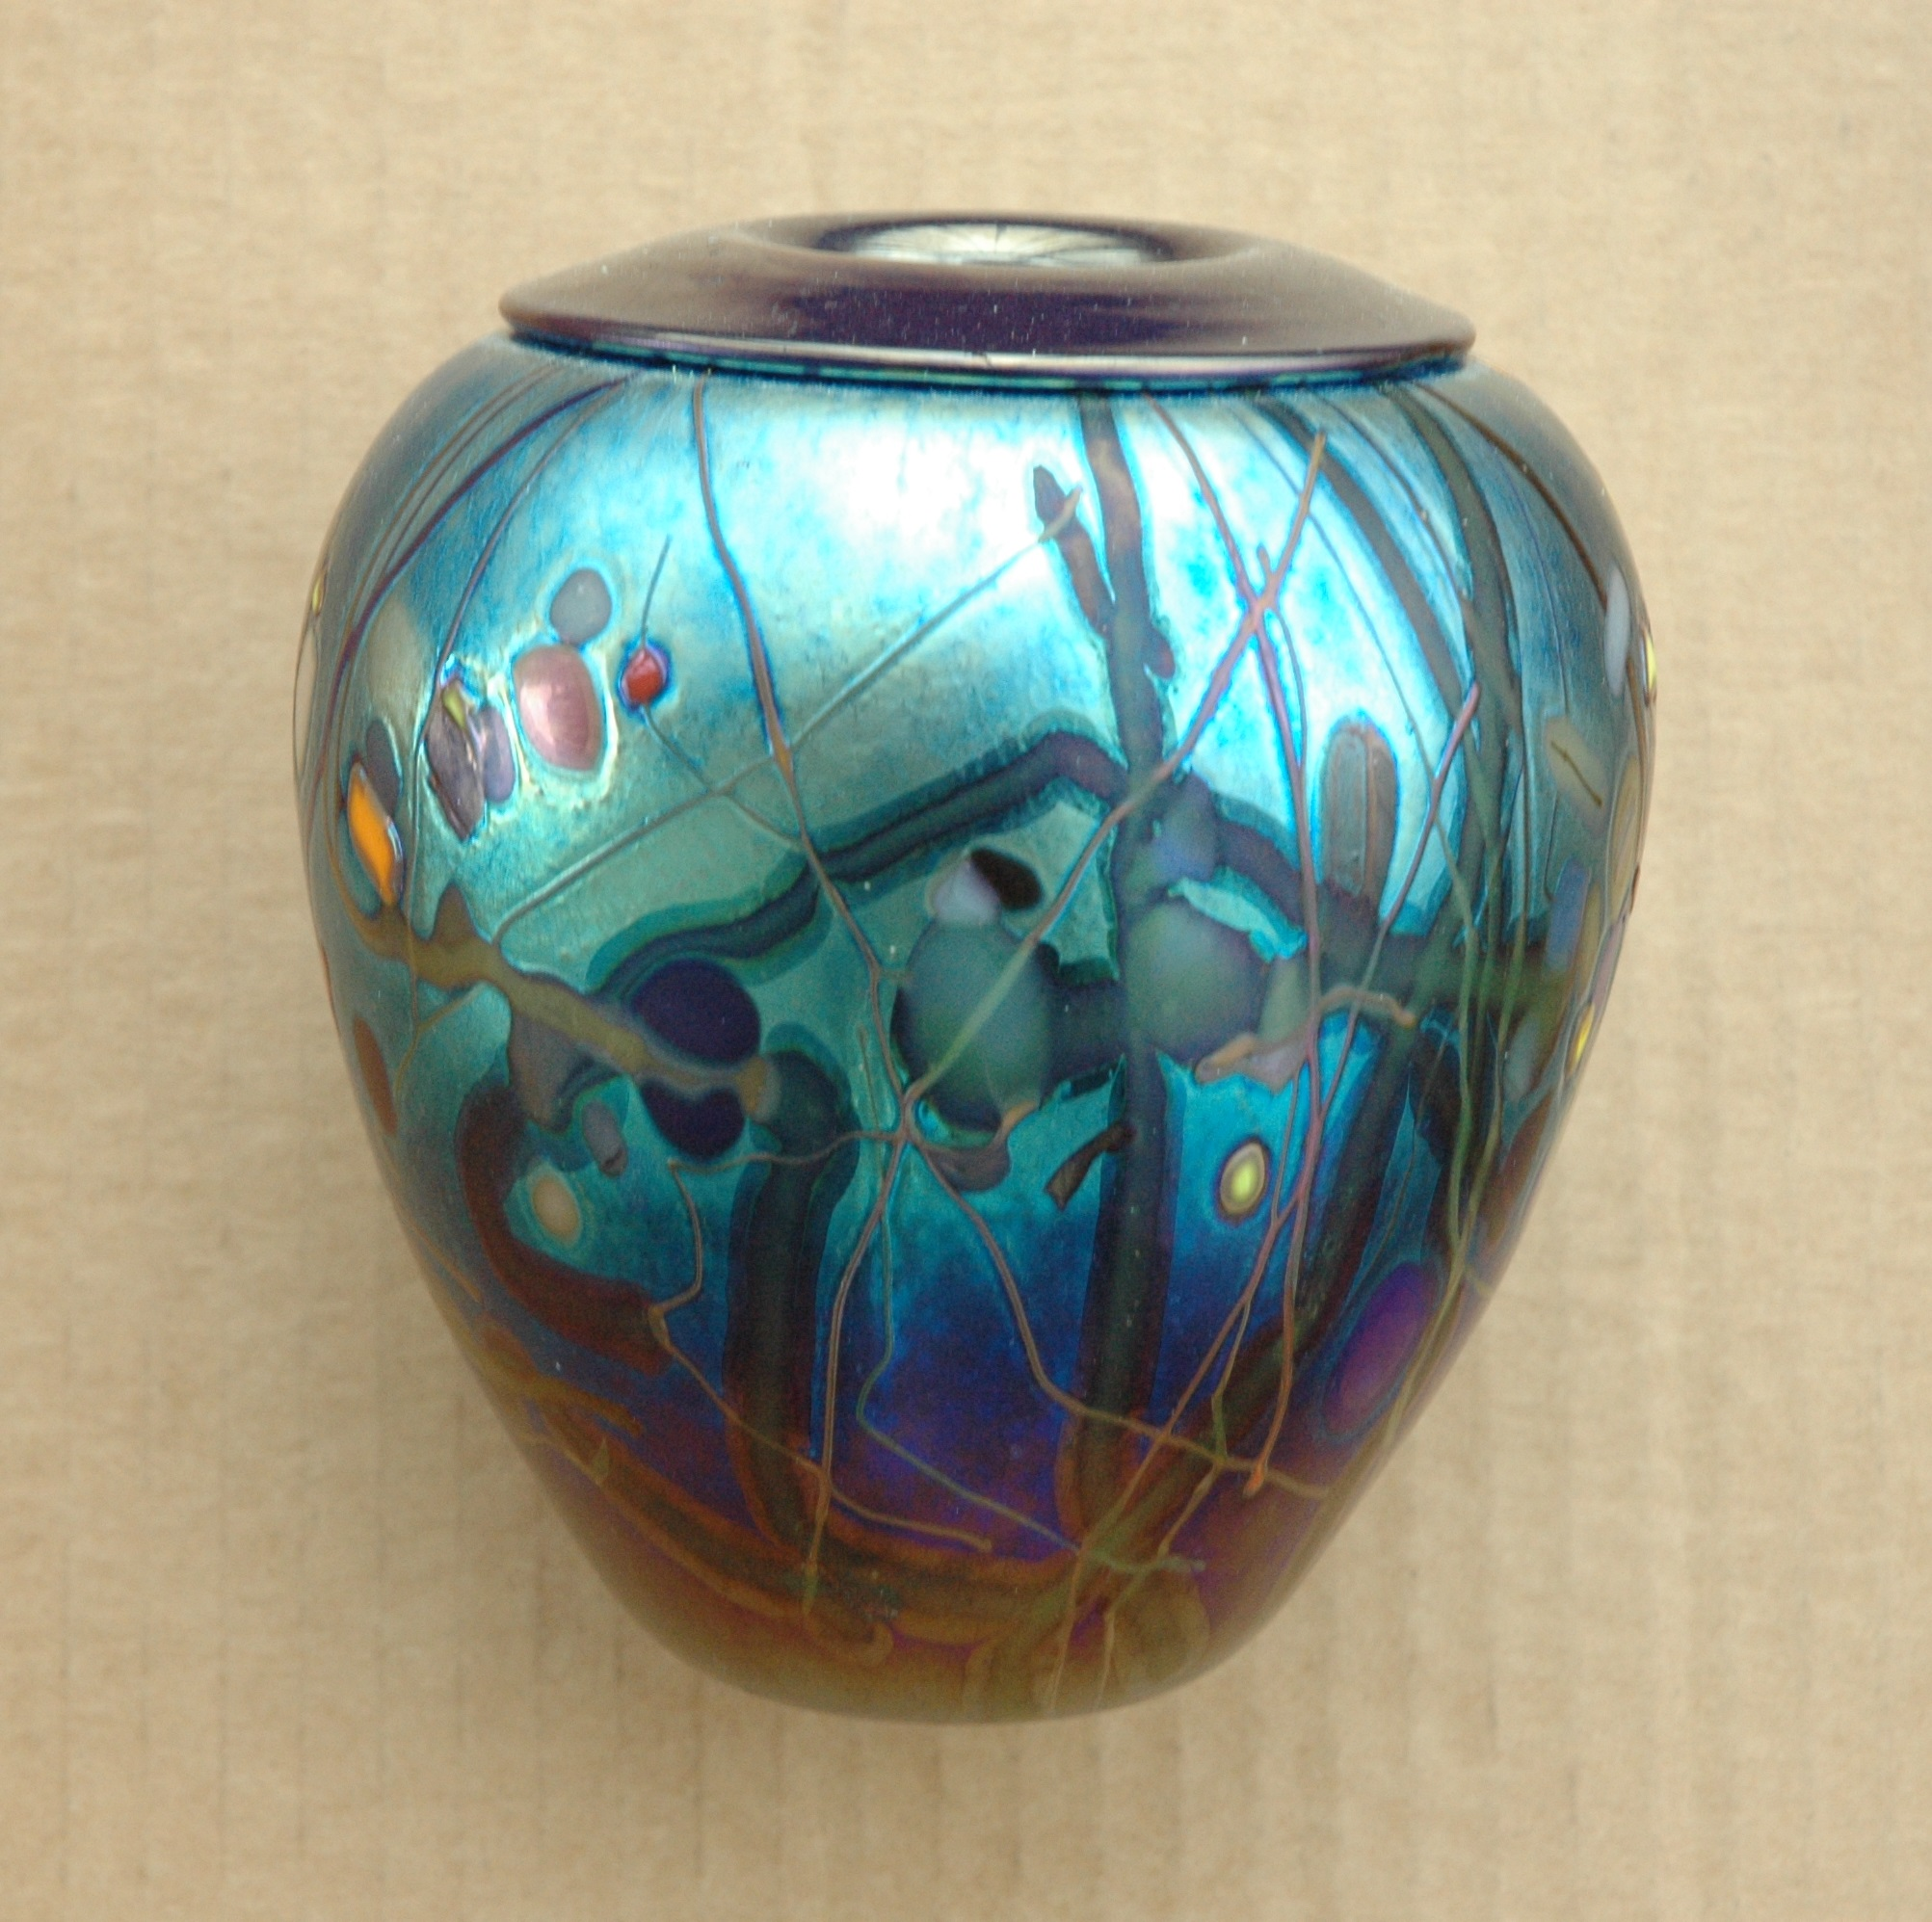
\includegraphics[width=0.15\textwidth]{interp/real_world_img/vase/vase}\\ \cline{1-5}
\multirow{3}{*}{\rotatebox[origin=c]{90}{appearance}}
  & textureless & textureless & textured & textured\\
  & diffuse & mixed d/s & diffuse & mixed d/s\\
  & bright & bright & dark/bright & dark/bright\\
\end{tabular}
\end{figure}

\end{frame}

%------------------------------------------------
\begin{frame}{Interpretation 1: demonstrative result}

accurate description $\Rightarrow$ successful result?

\begin{figure}
\centering
\includegraphics[width=0.8\textwidth]{images/interp1.pdf}
\end{figure}

\begin{exampleblock}{Comparison to baseline result}
\begin{itemize}
\item accuracy: higher quality
\item completenss: no incomplete holes
\end{itemize}
\end{exampleblock}

\end{frame}

%------------------------------------------------
\begin{frame}{Interpretation 2: demonstrative result}

less accurate description $\Rightarrow$ less successful result?

\begin{figure}
\centering
\includegraphics[width=0.8\textwidth]{images/interp2.pdf}
\end{figure}

\begin{exampleblock}{Comparison to baseline result}
\begin{itemize}
\item completenss: has incomplete holes
\end{itemize}
\end{exampleblock}

\end{frame}

%------------------------------------------------
\begin{frame}{Interpretation 2: demonstrative result (cont'd)}

less accurate description $\Rightarrow$ less successful result?

\begin{figure}
\centering
\includegraphics[width=0.8\textwidth]{images/interp2_1.pdf}
\end{figure}

\begin{exampleblock}{Comparison to baseline result}
\begin{itemize}
\item accuracy: higher quality
\item completenss: no incomplete holes
\end{itemize}
\end{exampleblock}

\end{frame}

%------------------------------------------------
\begin{frame}{Interpretation 3: demonstrative result}

inaccurate description $\Rightarrow$ poor result?

\begin{figure}
\centering
\includegraphics[width=0.8\textwidth]{images/interp3.pdf}
\end{figure}

\begin{exampleblock}{Summary}
\begin{itemize}
\item accuracy/completeness: surface rougher, poorer
\end{itemize}
\end{exampleblock}

\end{frame}

%------------------------------------------------
\begin{frame}{Interpretation: overview}

\begin{figure}
\centering
\includegraphics[width=0.8\textwidth]{images/result_summary.pdf}
\end{figure}

\end{frame}

%------------------------------------------------
\begin{frame}{Interpretation: summary}

\begin{exampleblock}{}
\begin{itemize}
\item We have demonstrated that it is achievable to design an description-based interface so that a successful reconstruction result is obtained given a description of problem condition, without knowledge of which algorithm to use;
\item The reconstruction result improves as the accuracy of the description increases.
% \item Algorithm chosen by the interpreter given a less accurate description may or may not achieve a poor result;
% \item It depends if the return algorithms has at least an overlapping with those returned if given accurate description;
% \item Algorithm chosen by the interpreter given inaccurate description have a higher probability of achieving a poorer result.
\end{itemize}
\end{exampleblock}

\end{frame}

%------------------------------------------------
\begin{frame}{Interpreter: results}

\begin{figure}
\centering
\includegraphics[width=0.9\textwidth]{images/3d_recon_interface_2.pdf}
\end{figure}

\begin{exampleblock}{Strengths}
  \begin{itemize}
    \item \textbf{Algorithms}: description of appearance, no vision background needed, embeding new algorithms is easy;
    \item \textbf{Parameters}: property parameters are perceptually interpretable\& meaningful;
    \item \textbf{Approach}: no \textit{trial-and-error}.
  \end{itemize}
\end{exampleblock}

\end{frame}

%------------------------------------------------
\section{Conclusions}
%------------------------------------------------
\begin{frame}{Conclusions}

\begin{itemize}
\item The proposed description is able to give correct reconstruction for non-concave objects;
\item The solution produced by the interface gets better as the description becomes more accurate, and vice versa;
\item Using the simple descriptive language and proof-of-concept interpreter, we demonstrate the possibility of using descriptive properties to hide algorithmic details;
\item To deal with more complicated objects, we need more complicated properties, or ways to describe the objects, but the challenge is the easy mathematical representation might not be available.
\end{itemize}

\end{frame}

%------------------------------------------------
\begin{frame}{Recommendations and Future directions}

\begin{itemize}
\item Develop automated approach to derive description from images;
\item Develop more sophisticated geometric model to incorporate objects with complex geometry;
\end{itemize}

\end{frame}

%------------------------------------------------
\begin{frame}[standout]

Computer vision should focus on more than \\just algorithms, but easier accessibility.

\end{frame}

%------------------------------------------------
% Additional slides
%------------------------------------------------

%------------------------------------------------
\begin{frame}{Mapping: dataset}

\begin{exampleblock}{creation of dataset}
\begin{itemize}
\item We need a dataset contains object with varied visual and geometric properties;
\item Generate the dataset using physic-based renderer.
\end{itemize}
\end{exampleblock}

% \begin{exampleblock}{example of synthetic object}
% \begin{figure}
% \centering
% 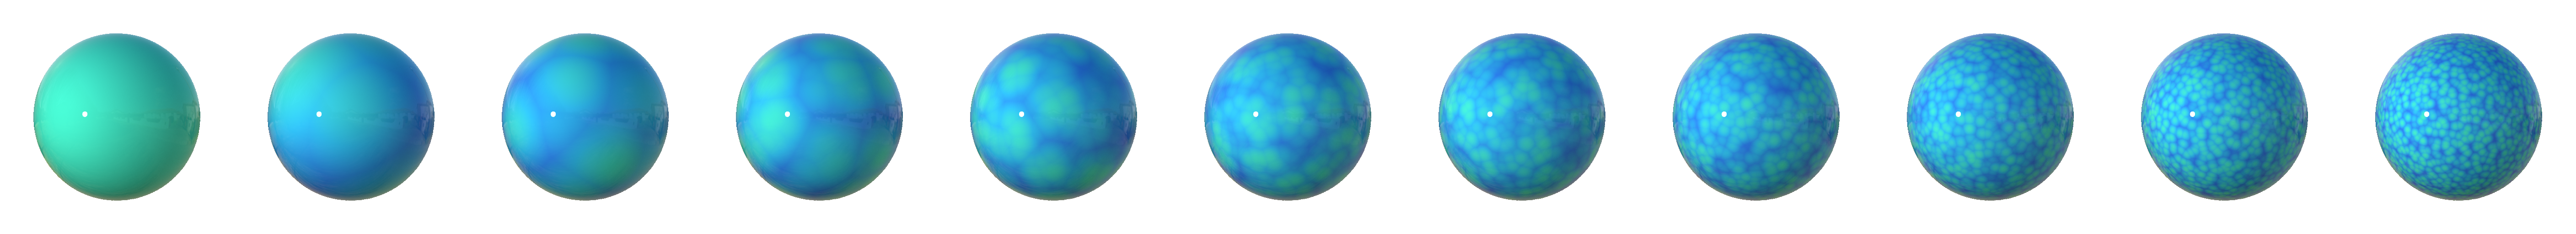
\includegraphics[width=0.8\textwidth]{mapping/setup/tex}
% \end{figure}
% \end{exampleblock}

\end{frame}

%------------------------------------------------
\begin{frame}{Mapping: interesting observations}

% We provide key observations that can be theoretically justified by theory to demonstrate the insights that could be obtained from the mapping.

\begin{exampleblock}{1. PMVS can work on specular surfaces provided the surface highly textured}
\begin{figure}
\begin{tabular}{ccc}
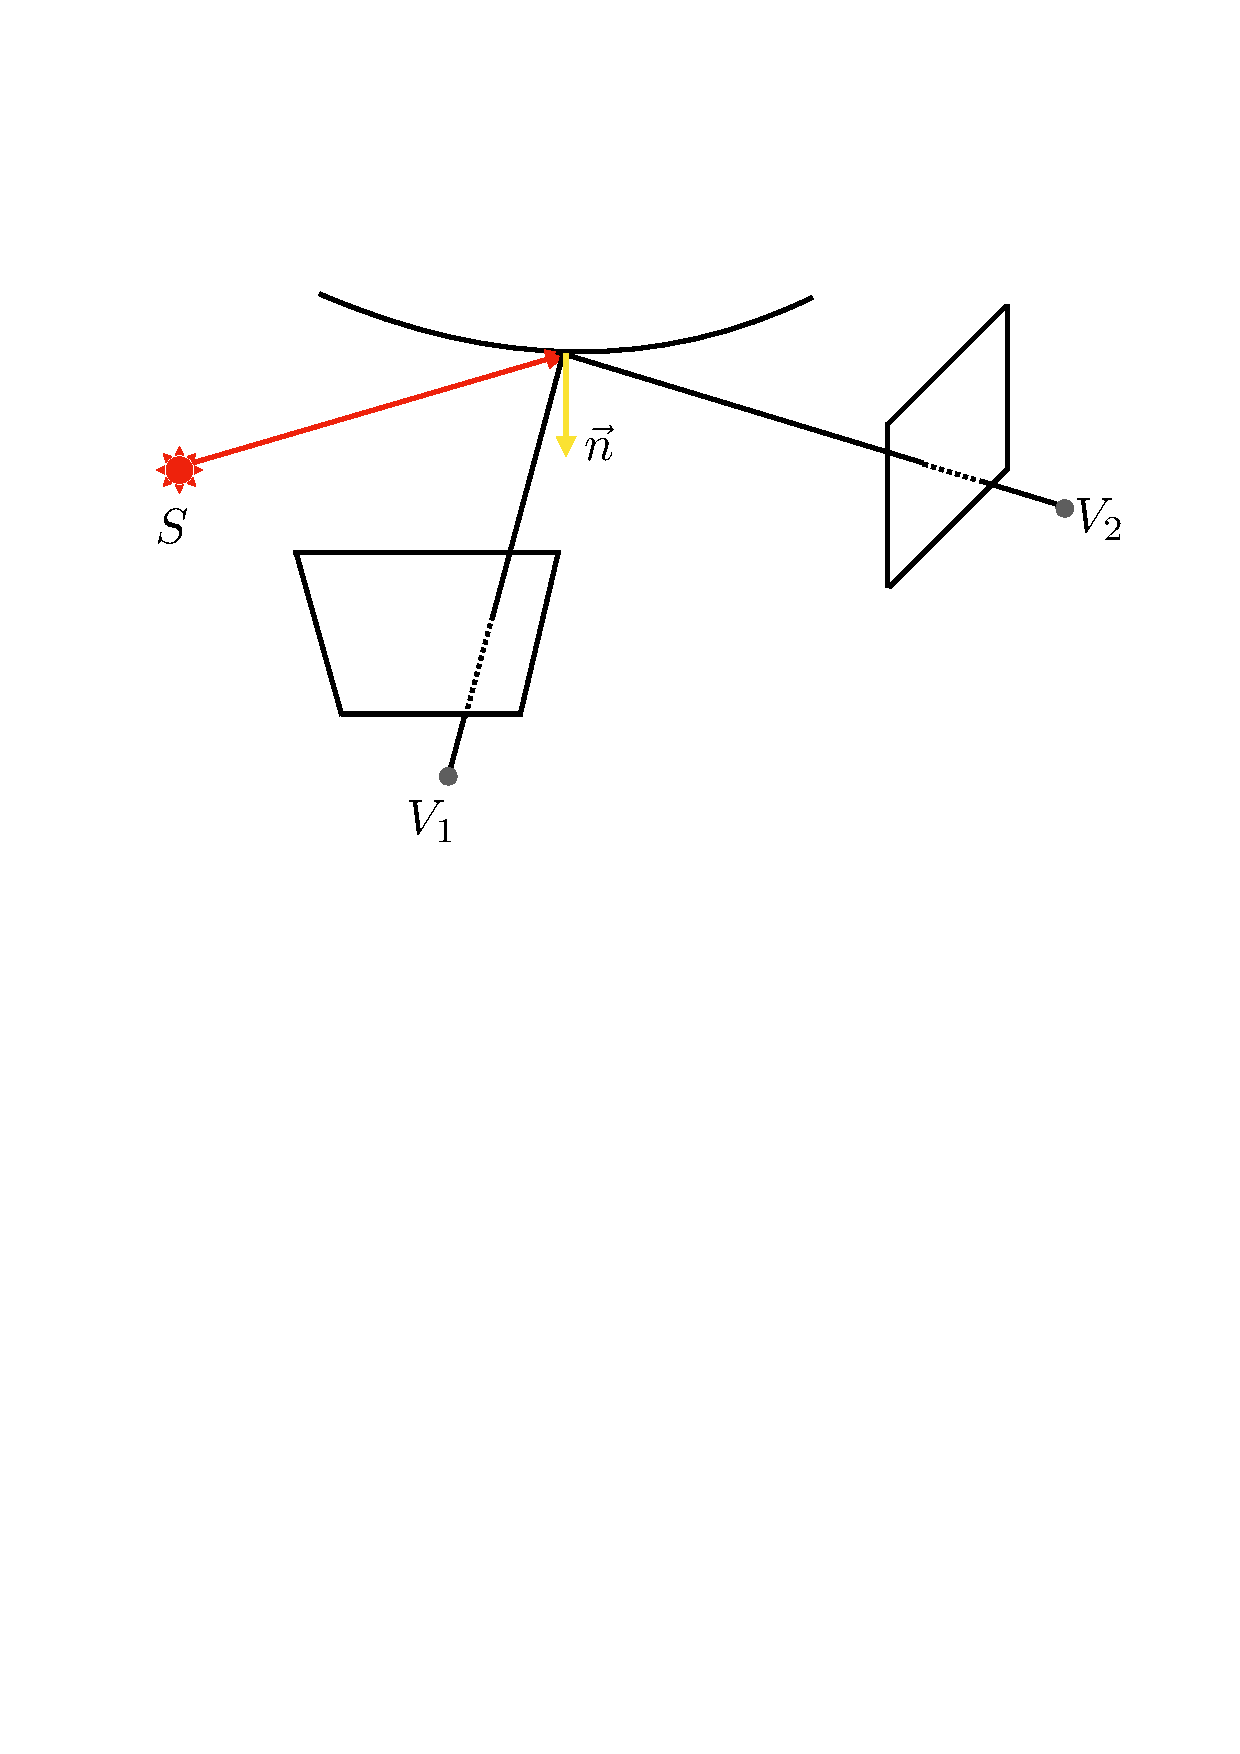
\includegraphics[width=0.22\textwidth]{mapping/mvs_spec/mvs_spec}&
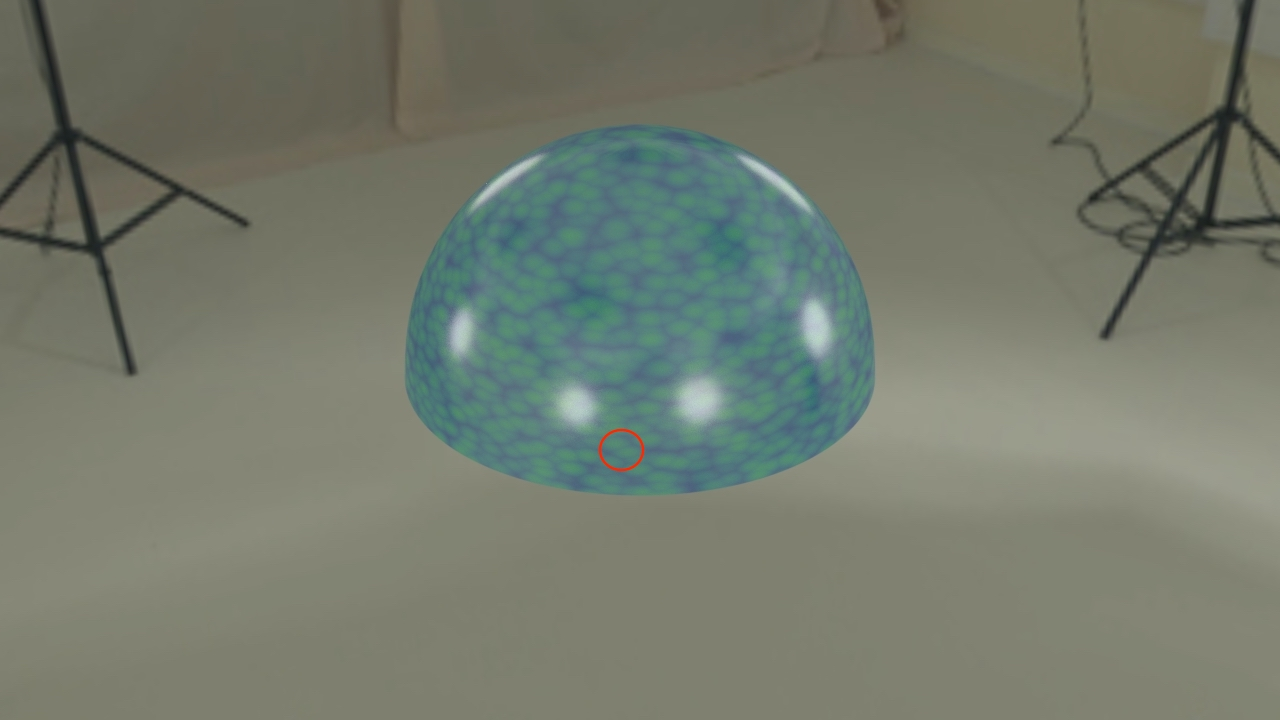
\includegraphics[width=0.22\textwidth]{mapping/mvs_spec/mvs_spec_01}&
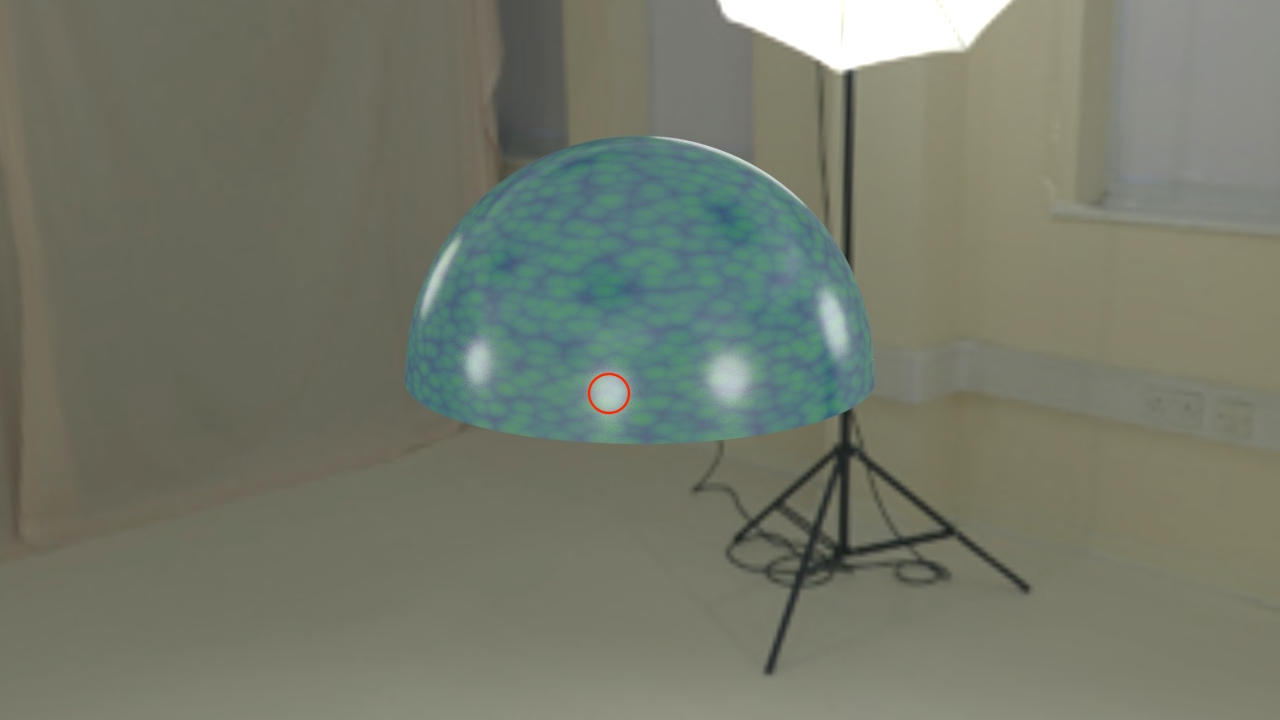
\includegraphics[width=0.22\textwidth]{mapping/mvs_spec/mvs_spec_00}\\
% (a). Image formation & (b) $V_1$ & (c) $V_2$\\
\end{tabular}
\end{figure}
\end{exampleblock}

\begin{exampleblock}{2. EPS and GSL fails on highly specular surfaces, and a blurred specular area leads to worse results.}
\begin{figure}
\begin{tabular}{ccc}
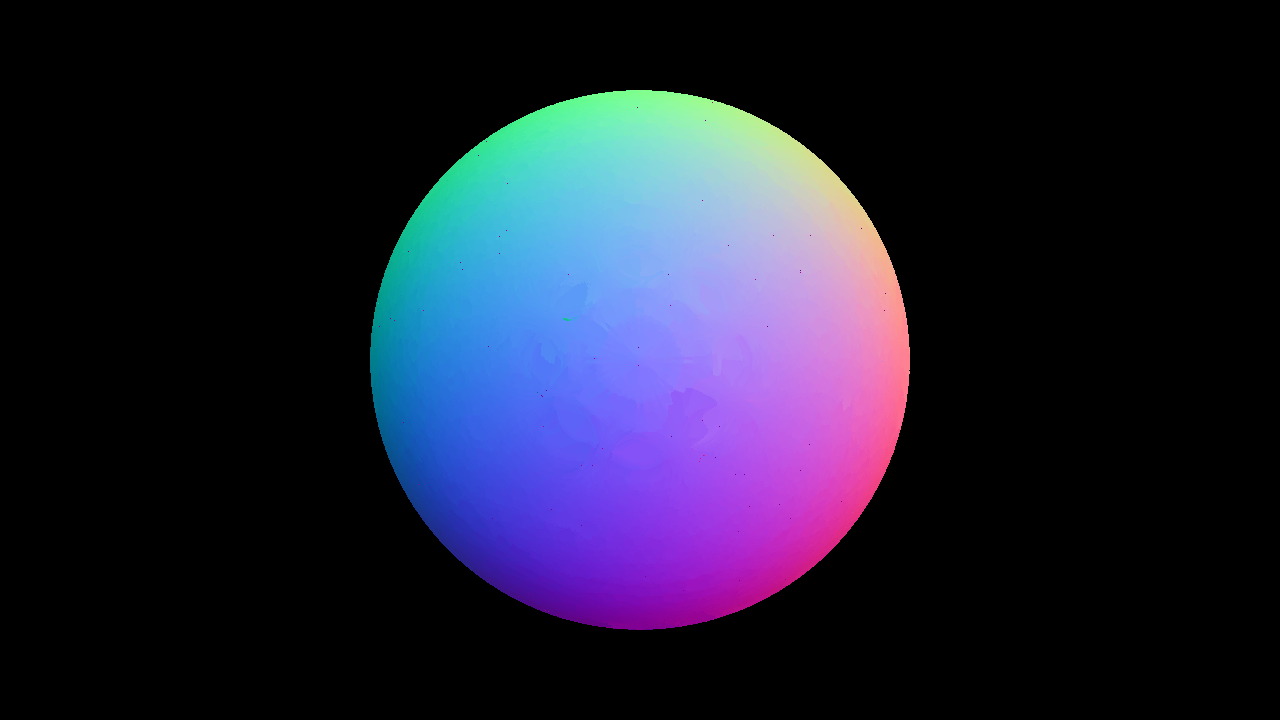
\includegraphics[width=0.15\textwidth]{mapping/ps_spec_rough/0802_normal}&
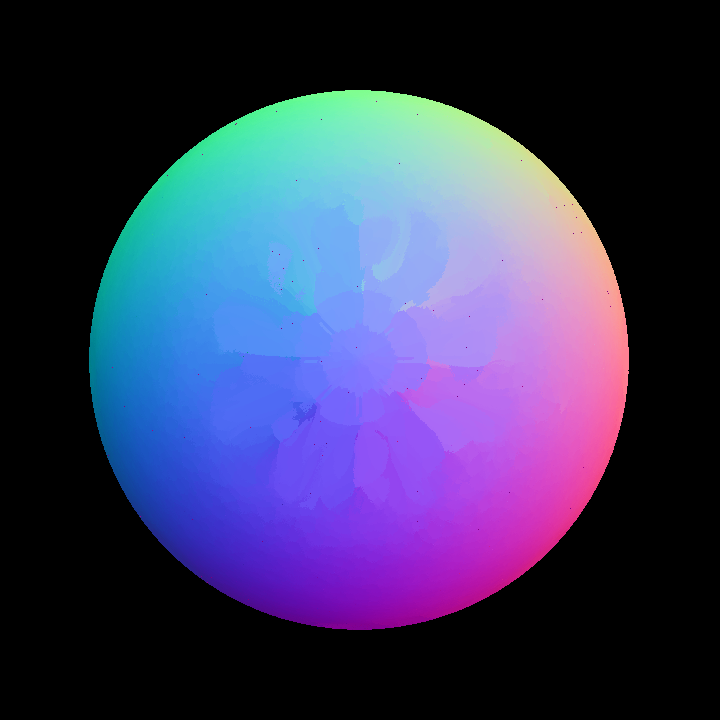
\includegraphics[width=0.15\textwidth]{mapping/ps_spec_rough/0805_normal}&
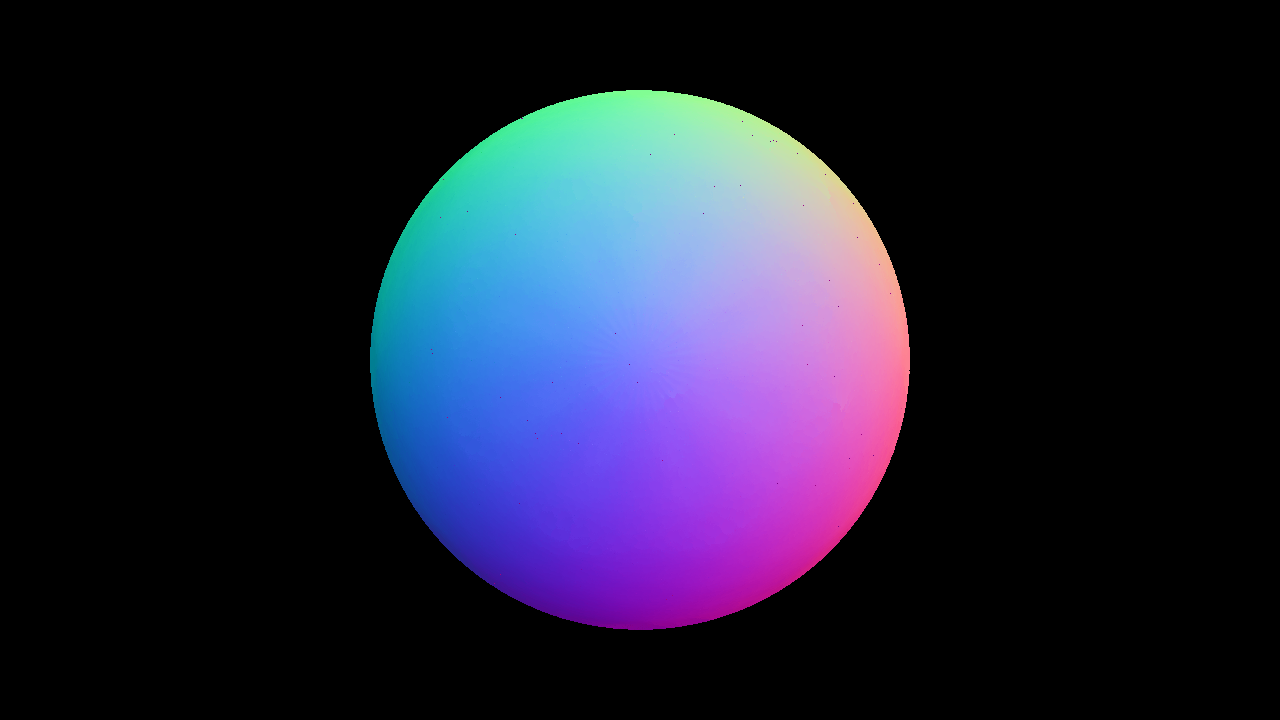
\includegraphics[width=0.15\textwidth]{mapping/ps_spec_rough/0808_normal}\\
(a). rough: 0.2 & (b). rough: 0.5 & (c). rough: 0.8
\end{tabular}
\end{figure}
\end{exampleblock}

\end{frame}

%------------------------------------------------
% \begin{frame}{Mapping: notable findings 1}

% \begin{figure}[!htbp]
% \begin{tabular}{cc}
% \includegraphics[width=0.22\textwidth]{mapping/pairwise/mvs_tex_spec}&
% \includegraphics[width=0.22\textwidth]{mapping/mvs_spec/mvs_spec}\\
% (a). Algo. performance & (b) Image formation\\
% \includegraphics[width=0.22\textwidth]{mapping/mvs_spec/mvs_spec_01}&
% \includegraphics[width=0.22\textwidth]{mapping/mvs_spec/mvs_spec_00}\\
% (c) $V_1$ & (d) $V_2$\\
% \end{tabular}
% \caption{(a) shows the algorithm performance w.r.t. texture and specularity. (b) shows the reflection of light off a specular surface. $V_1$ received the diffuse component while $V_2$ receives the specular component. (c), (d) shows the images observed from these two views. The specular area (red circle) observed in $V_2$ is visible in $V_1$.}
% \end{figure}

% \end{frame}

%------------------------------------------------
% \begin{frame}{Mapping: notable findings 2}

% \begin{figure}[!htbp]
% \centering
% \begin{tabular}{c|ccc}
%   Image & Normal map & Height map & Angular error\\
%   \hline\\
%   \includegraphics[width=0.12\textwidth]{mapping/ps_spec_rough/0802_0001}&
%   \includegraphics[width=0.12\textwidth]{mapping/ps_spec_rough/0802_normal}&
%   \includegraphics[width=0.15\textwidth]{images/0802_dmap}&
%   \includegraphics[width=0.05\textwidth]{mapping/ps_spec_rough/0802_ang_error}\\
%   & (a). rough: 0.2\\
%   \includegraphics[width=0.12\textwidth]{mapping/ps_spec_rough/0805_0001}&
%   \includegraphics[width=0.12\textwidth]{mapping/ps_spec_rough/0805_normal}&
%   \includegraphics[width=0.15\textwidth]{images/0805_dmap}&
%   \includegraphics[width=0.05\textwidth]{mapping/ps_spec_rough/0805_ang_error}\\
%   & (b). rough: 0.5\\
%   \includegraphics[width=0.12\textwidth]{mapping/ps_spec_rough/0808_0001}&
%   \includegraphics[width=0.12\textwidth]{mapping/ps_spec_rough/0808_normal}&
%   \includegraphics[width=0.15\textwidth]{images/0808_dmap}&
%   \includegraphics[width=0.05\textwidth]{mapping/ps_spec_rough/0808_ang_error}\\
%   & (c). rough: 0.8\\
% \end{tabular}
% \caption{The effect of roughness on PS. Albedo is set as 0.8, and specular is set as 0.8. (b) demonstrates that a medium level roughness would lead to worse normal estimation since it blurs the specular lobe.}
% \end{figure}

% \end{frame}

%------------------------------------------------
% \begin{frame}{Mapping: notable findings 3}

% \begin{figure}[!htbp]
% \centering
% \begin{tabular}{ccc}
% \includegraphics[width=0.25\textwidth]{trash/mapping/sl_spec_rough/sl_00050202}&
% \includegraphics[width=0.25\textwidth]{trash/mapping/sl_spec_rough/sl_00050502}&
% \includegraphics[width=0.25\textwidth]{trash/mapping/sl_spec_rough/sl_00050802}\\
% (a) specular: 0.2 & (b) specular: 0.5 & (c) specular: 0.8\\
% \includegraphics[width=0.25\textwidth]{trash/mapping/sl_spec_rough/sl_00050802}&
% \includegraphics[width=0.25\textwidth]{trash/mapping/sl_spec_rough/sl_00050805}&
% \includegraphics[width=0.25\textwidth]{trash/mapping/sl_spec_rough/sl_00050808}\\
% (d) roughness: 0.2 & (e) roughness: 0.5 & (f) roughness: 0.8\\
% \end{tabular}
% \caption{(a)-(c): the roughness is set as 0.2, and specular has a negative effect on completeness; (d)-(e): the specular is set as 0.8, roughness has a positive effect on completeness.}
% \end{figure}

% \end{frame}

%------------------------------------------------
\begin{frame}{Interpretation 1: more results}

\begin{figure}
\centering
\begin{tabular}{lcccc}
\parbox[t]{2mm}{\rotatebox[origin=c]{90}{Algo}}
& GSL & EPS & GSL & PMVS \\
\midrule
\parbox[t]{2mm}{\rotatebox[origin=c]{90}{Result}}
& \raisebox{-.5\height}{\includegraphics[width=0.15\textwidth]{interp/synth_interp/beethoven_sl}}
& \raisebox{-.5\height}{\includegraphics[width=0.15\textwidth]{interp/synth_interp/vase0_ps}}
& \raisebox{-.5\height}{\includegraphics[width=0.15\textwidth]{interp/synth_interp/barrel_sl}}
& \raisebox{-.5\height}{\includegraphics[width=0.15\textwidth]{interp/synth_interp/vase1_mvs}}\\
\parbox[t]{2mm}{\rotatebox[origin=c]{90}{BL result}}
& \raisebox{-.5\height}{\includegraphics[width=0.15\textwidth]{interp/synth_interp/beethoven_vh}}
& \raisebox{-.5\height}{\includegraphics[width=0.15\textwidth]{interp/synth_interp/vase0_vh}}
& \raisebox{-.5\height}{\includegraphics[width=0.15\textwidth]{interp/synth_interp/barrel_vh}}
& \raisebox{-.5\height}{\includegraphics[width=0.15\textwidth]{interp/synth_interp/vase1_vh}}\\
\midrule
\parbox[t]{2mm}{\rotatebox[origin=c]{90}{Result}}
& \raisebox{-.5\height}{\includegraphics[width=0.15\textwidth]{interp/real_interp/statue/statue_sl}}
& \raisebox{-.5\height}{\includegraphics[width=0.15\textwidth]{interp/real_interp/cup/cup_ps}}
& \raisebox{-.5\height}{\includegraphics[width=0.15\textwidth]{interp/real_interp/pot/pot_sl}}
& \raisebox{-.5\height}{\includegraphics[width=0.15\textwidth]{interp/real_interp/vase/vase_mvs}}\\
\parbox[t]{2mm}{\rotatebox[origin=c]{90}{BL result}}
& \raisebox{-.5\height}{\includegraphics[width=0.15\textwidth]{interp/real_interp/statue/statue_sc}}
& \raisebox{-.5\height}{\includegraphics[width=0.15\textwidth]{interp/real_interp/cup/cup_sc}}
& \raisebox{-.5\height}{\includegraphics[width=0.15\textwidth]{interp/real_interp/pot/pot_sc}}
& \raisebox{-.5\height}{\includegraphics[width=0.15\textwidth]{interp/real_interp/vase/vase_sc}}\\
\end{tabular}
\end{figure}

\end{frame}

%------------------------------------------------
\begin{frame}{Interpretation 2: demonstrative result (cont'd)}

\begin{figure}
\centering
\includegraphics[width=\textwidth]{images/interp2_2.pdf}
\end{figure}

\end{frame}

%------------------------------------------------
\begin{frame}{Interpretation 2: more results}

\begin{figure}
\centering
\begin{tabular}{c|*{5}{l}}
Object & $Desc_1$ & $Desc_2$ & $Desc_3$ & $Desc_4$ & Correct Desc \\
\midrule
Desc & \tc{08}080802 & 02\tc{02}0802 & 0208\tc{02}02 & 020808\tc{08} & 02080802 \\
Algo & PMVS & BL & GSL & GSL & \tc{EPS}\\
vase0 & \raisebox{-.5\height}{\includegraphics[width=0.1\textwidth]{interp/synth_interp/vase0_mvs}} &
  \raisebox{-.5\height}{\includegraphics[width=0.1\textwidth]{interp/synth_interp/vase0_vh}} &
  \raisebox{-.5\height}{\includegraphics[width=0.1\textwidth]{interp/synth_interp/vase0_sl}} &
  \raisebox{-.5\height}{\includegraphics[width=0.1\textwidth]{interp/synth_interp/vase0_sl}} &
  \raisebox{-.5\height}{\includegraphics[width=0.1\textwidth]{interp/synth_interp/vase0_ps}}\\
cup & \raisebox{-.5\height}{\includegraphics[width=0.1\textwidth]{interp/real_interp/cup/cup_mvs}} &
  \raisebox{-.5\height}{\includegraphics[width=0.1\textwidth]{interp/real_interp/cup/cup_sc}} &
  \raisebox{-.5\height}{\includegraphics[width=0.1\textwidth]{interp/real_interp/cup/cup_sl}} &
  \raisebox{-.5\height}{\includegraphics[width=0.1\textwidth]{interp/real_interp/cup/cup_sl}} &
  \raisebox{-.5\height}{\includegraphics[width=0.1\textwidth]{interp/real_interp/cup/cup_ps}} \\
\midrule
Desc & \tc{08}080208 & 02\tc{02}0208 & 0208\tc{08}08 & 020802\tc{02} & 02080208 \\
\multirow{2}{*}{Algo} & GSL & EPS & GSL & GSL & EPS \\
& & & & & \tc{GSL} \\
bust & \raisebox{-.5\height}{\includegraphics[width=0.1\textwidth]{interp/synth_interp/beethoven_sl}} &
  \raisebox{-.5\height}{\includegraphics[width=0.1\textwidth]{interp/synth_interp/beethoven_ps}} &
  \raisebox{-.5\height}{\includegraphics[width=0.1\textwidth]{interp/synth_interp/beethoven_sl}} &
  \raisebox{-.5\height}{\includegraphics[width=0.1\textwidth]{interp/synth_interp/beethoven_sl}} &
  \raisebox{-.5\height}{\includegraphics[width=0.1\textwidth]{interp/synth_interp/beethoven_sl}}\\
statue & \raisebox{-.5\height}{\includegraphics[width=0.1\textwidth]{interp/real_interp/statue/statue_sl}} &
  \raisebox{-.5\height}{\includegraphics[width=0.1\textwidth]{interp/real_interp/statue/statue_ps}} &
  \raisebox{-.5\height}{\includegraphics[width=0.1\textwidth]{interp/real_interp/statue/statue_sl}} &
  \raisebox{-.5\height}{\includegraphics[width=0.1\textwidth]{interp/real_interp/statue/statue_sl}} &
  \raisebox{-.5\height}{\includegraphics[width=0.1\textwidth]{interp/real_interp/statue/statue_sl}} \\
\end{tabular}
\end{figure}

\end{frame}

%------------------------------------------------
\begin{frame}{Interpretation 3: more results}

\begin{figure}
\centering
\begin{tabular}{c*{4}{l}}
Object & Bust & Vase0 & Barrel & Vase1 \\
\midrule
\parbox[t]{2mm}{\multirow{4}{*}{\rotatebox[origin=c]{90}{Incorrect Desc}}} 
& 08020802 & 08020208 & 02020802 & 02020208 \\
& \tabitem\tc{BL} & \tabitem\tc{PMVS} & \tabitem\tc{BL} & \tabitem\tc{EPS} \\
&           & \tabitem EPS \\
& \includegraphics[width=0.1\textwidth]{interp/synth_interp/beethoven_vh}
& \includegraphics[width=0.1\textwidth]{interp/synth_interp/vase0_mvs}
& \includegraphics[width=0.1\textwidth]{interp/synth_interp/barrel_vh}
& \includegraphics[width=0.1\textwidth]{interp/synth_interp/vase1_ps} \\ \cline{1-5}
\parbox[t]{2mm}{\multirow{5}{*}{\rotatebox[origin=c]{90}{Correct Desc}}}
& 02080208 & 02080802 & 08080208 & 08080802 \\
& \tabitem EPS    & \tabitem\tc{EPS} & \tabitem PMVS    & \tabitem\tc{PMVS} \\
& \tabitem\tc{GSL}  &          & \tabitem EPS     & \tabitem EPS \\
&           &            & \tabitem\tc{GSL} & \\
& \includegraphics[width=0.1\textwidth]{interp/synth_interp/beethoven_sl}
& \includegraphics[width=0.1\textwidth]{interp/synth_interp/vase0_ps}
& \includegraphics[width=0.1\textwidth]{interp/synth_interp/barrel_sl}
& \includegraphics[width=0.1\textwidth]{interp/synth_interp/vase1_mvs} \\
\end{tabular}
\end{figure}

\end{frame}

%------------------------------------------------
\begin{frame}{Interpretation 3: more results (cont'd)}

\begin{figure}
\centering
\begin{tabular}{c*{4}{l}}
Object & Statue & Cup & Pot & Vase \\
\midrule
\parbox[t]{2mm}{\multirow{4}{*}{\rotatebox[origin=c]{90}{Incorrect Desc}}}
& 08020802 & 08020208 & 02020802 & 02020208 \\
& \tabitem\tc{BL} & \tabitem\tc{PMVS} & \tabitem\tc{BL} & \tabitem\tc{EPS} \\
&           & \tabitem EPS \\
& \includegraphics[width=0.1\textwidth]{interp/real_interp/statue/statue_sc}
& \includegraphics[width=0.1\textwidth]{interp/real_interp/cup/cup_mvs}
& \includegraphics[width=0.1\textwidth]{interp/real_interp/pot/pot_sc}
& \includegraphics[width=0.1\textwidth]{interp/real_interp/vase/vase_ps} \\ \cline{1-5}
\parbox[t]{2mm}{\multirow{5}{*}{\rotatebox[origin=c]{90}{Correct Desc}}}
& 02080208 & 02080802 & 08080208 & 08080802 \\
& \tabitem EPS    & \tabitem\tc{EPS} & \tabitem PMVS    & \tabitem\tc{PMVS} \\
& \tabitem\tc{GSL}  &          & \tabitem EPS     & \tabitem EPS \\
&           &            & \tabitem\tc{GSL} & \\
& \includegraphics[width=0.1\textwidth]{interp/real_interp/statue/statue_sl}
& \includegraphics[width=0.1\textwidth]{interp/real_interp/cup/cup_ps}
& \includegraphics[width=0.1\textwidth]{interp/real_interp/pot/pot_sl}
& \includegraphics[width=0.1\textwidth]{interp/real_interp/vase/vase_mvs} \\
\end{tabular}
\end{figure}

\end{frame}

\end{document}
